\cotefile{136}
\scanpage{189}
\begin{center}- \mspage{64} -\end{center}
\margin{IX}

une propriété nettement plus forte que celle énoncée dans 5.7, qui pourra alors servir de caractérisation intrinsèque de la partie fixe de $T_p(A_K)$ (en termes de la seule structure de pro-groupe de Barsotti-Tate de $T_p(A_K)$), - du moins dans le cas d'inégales caractéristiques :

\uline{Théorème} 5.8. (M. RAYNAUD). \uline{Soit} $A_K$ \uline{un schéma abélien à réduction semi-stable sur le corps des fonctions} $K$ \uline{d'un trait hensélien} $S$. \uline{Soit} $\ell$ \uline{un nombre premier} (\uline{le cas intéressant étant celui où} $\ell=p$), \uline{et considérons le pro-}$\ell$\uline{-groupe de Barsotti-Tate} $X_\eta=T_\ell(A_K)$ \uline{et sa} ``\uline{partie fixe}''$X_\eta^f$, \uline{qui est la fibre générique du} pro-$\ell$\uline{-groupe de Barsotti-Tate} $X^f=T_\ell(A^{\unsure{0|o}})^f$. \uline{Supposons}, \uline{si} $\ell=p$, \uline{qu'on ait} $\mathrm{car.}\ K=0$(\uline{de sorte que nous disposons sur} $S$ \uline{du théorème de TATE} [33, th.4]).\uline{Soit} $F$ \uline{un pro-}$\ell$\uline{-groupe de Barsotti-Tate sur} $S$. \uline{Alors tout homomorphisme} $F_\eta\longrightarrow X_\eta$ \uline{se factorise par} $X_\eta^f$.

Passant aux ind-$\ell$-groupes associés aux pro-$\ell$-groupes de Barsotti-Tate envisagés,l'énoncé précédent devient équivalent au suivant, grâce au théorème cité de TATE :

\uline{Corollaire} 5.9. \uline{Si} $F$ \uline{est un} ind-$\ell$\uline{-groupe de Barsotti-Tate}, \uline{alors tout homomorphisme} $u_\eta:F_\eta\longrightarrow A_\eta$ \uline{se prolonge} (\uline{de façon unique}) \uline{en un homomorphisme} $u:F\longrightarrow A$.

En d'autres termes, la propriété ``néronienne'' caractéristique (1.1.2) du modèle de Néron reste valable pour des homomorphismes de ind-schémas en groupes de Barsotti-Tate, sans hypothèse de lissité sur celui-ci. (Seul le cas des groupes ind-étales résulterait directement de la définition.)

\margin{382}
\margin{382}
\margin{188}

\scanpage{190}
\[
\boxed{\boxed{\beta(A_1)=T}}\quad\text{i.e.}\quad A_1(T)=T
\]
\deleted{\unsure{Donnons}} Considérons
\deleted{\unsure{Du}}
\[
A_1-X_0=\varphi_0^0(X_0)-X_0=-(\varphi_0^0(X_1)-X_1)=f\in\mathcal A_1^0
\]
(où $\varphi_0(x)$ est la composante de $\varphi(x)$ \unsure{suivant}
\[
S\{X_0\}\simeq\overbrace{k\{T\}}\{X_0,X_1\}/(X_0+X_1-T)_{\mathrm{pd}}
\]
dans
\[
\mathcal A_1=\underbrace{S\{X_0\}}_{\mathcal A_1^0}+\underbrace{S\{X_0\}\,dX_0}_{\mathcal A_1^1}\simeq S\{X_1\}+S\{X_1\}\,dX_1
\]
)

[\unsure{NB.} Comme $X_1=T-X_0$, \unsure{on a}
\[
\varphi_0^0(X_1)=\varphi_0^0(T)-\varphi_0^0(X_0)\inserted{=T-\varphi_0^0(X_0)},\quad\text{d'où}\quad\varphi_0^0(X_1)-X_1=X_0-\varphi_0^0(X_0)
\]
]

Alors la \unsure{conjonction} des conditions $A_1(X_0)=0$ et $A_1(T)=T$ s'écrit aussi
\[
f\in(X_0)_{\mathrm{pd}}\cap(X_1)_{\mathrm{pd}}
\]
donc, si \unsure{on interprète} $\mathcal A_1^0$ comme un \deleted{\unsure{quotient de}} $k\{X_0,X_1\}$, cela \unsure{signifie} qu'on doit avoir
\[
\boxed{f=\sum_{i,j\ge\text{\uuline{1}}}\deleted{\unsure{a_{ij}}}f_{ij}X_0^{(i)}X_1^{(j)}}\qquad f_{ij}\in k
\]
d'où un résumé
\deleted{$\unsure{\mathcal A_T=} $}

\uline{Prop.} Les endom. $\varphi$ de la $S$-algèbre diff.
\[
\mathcal A_1\simeq S\{X_0,X_1,dX_0,dX_1\}/(X_0+X_1-T,dX_0\unsure{-|+}dX_1)_{\mathrm{pd}},
\]
(où $S=k\{T\}$ avec ses puiss. div.) qui sont compatibles aux deux augm. $\alpha,\beta$
\[
\mathcal A_1\unsure{-|\longrightarrow}S\qquad(\alpha(X_0)=0,\alpha(X_1)=T;\ \beta(X_0)=T,\beta(X_1)=0)
\]
sont donnés exactement par les \unsure{systèmes}
\[
f\in\mathcal A_1^0\simeq k\{X_0,X_1\}
\]
avec
\[
f\in\operatorname{Ker}(k\{X_0,X_1\}\to k\{X_0\})\cap\operatorname{Ker}(k\{X_0,X_1\}\to k\{X_1\})
\]
i.e.
\[
\boxed{f=\sum_{i,j\ge1}a_{ij}X_0^{(i)}X_1^{(j)}}
\]
\margin{189}

\scanpage{191}
\margin{\unsure{1}}
\begin{center}- \mspage{62} -\end{center}
\margin{IX}
\margin{$=$}
\margin{-}

où on se rappellera que les groupes $T_\ell(A_K)^f$ et $T_\ell(A'_K)^f$ qui figurent au second membre sont les restrictions à $\eta$ de pro-$\ell$-groupes de Barsotti-Tate définis sur $S$, $T_\ell(A^{\unsure{0|o}})^f$ et $T_\ell(A'^{\unsure{0|o}})^f$ respectivement ; la lettre $D$ désigne ici les duals au sens des pro-groupes de Barsotti-Tate, savoir $\operatorname{\uline{Hom}}(-,\mathbb Z_\ell(1))$. Ainsi :

\uline{Proposition} 5.6. \uline{Supposons} $S$ \uline{complet et que} $A_K$ \uline{ait réduction semi-stable sur} $S$. \uline{Alors pour tout nombre premier} $\ell$ (\uline{qui peut être égal à la caractéristique résiduelle de} $S$), \uline{le pro-}$\ell$\uline{-groupe de Barsotti-Tate} $T_\ell(A_K)^t$ \uline{est la fibre générique d'un pro-groupe de Barsotti-Tate sur} $S$, ``\uline{de type torique}'', \uline{donné par} (5.5.7), \uline{tandis que} $T_\ell(A_K)/T_\ell(A_K)^f$ \uline{est la fibre générique d'un pro-groupe de Barsotti-Tate sur} $S$ \uline{de type pro-étale}, \uline{donné par} (5.5.8). \uline{Enfin les groupes} $T_\ell(A_K)^f$ \uline{et} $T_\ell(A_K)/T_\ell(A_K)^t$ \uline{sont les fibres génériques de pro-groupes de Barsotti-Tate définis sur} $S$, \uline{égaux respectivement à} $T_\ell(A^{\unsure{0|o}})^f$ \uline{et à} $D(T_\ell(A'^{\unsure{0|o}})^f)\unsure{-|=}\operatorname{\uline{Hom}}(T_\ell(A'^{\unsure{0|o}})^f,\mathbb Z_\ell(1))$.

5.6.1. On notera qu'il revient au même pour le revêtement étale $S'$ de déployer $T_\ell(A_K)^t$ ou de déployer $T_\ell(A_K)/T_\ell(A_K)^f$, car cela signifie respectivement que $S'$ déploie les groupes constants tordus $\underline M$ et \uline{$M'$}, or ceux-ci sont isogènes, puisque $T_{\unsure{o|0}}$ et $T'_{\unsure{o|0}}$ le sont. On voit en même temps qu'il existe une plus petite extension étale $S'$ de $S$ qui fait l'affaire.

Signalons aussi la conséquence facile suivante des définitions de 2.2.3 :

\margin{380}
\margin{-}
\margin{380}
\margin{190}

\scanpage{192}
et les
\[
\boxed{B_i\in\mathcal A_1^0=k\{X_0,X_1\}\qquad(i\ge0)}
\]
par les formules
\[
\begin{cases}
\varphi(X_0^{(i)})=(X_0+f)^{(i)}+B_i\,dX_0\\
\varphi(dX_0)=1+df
\end{cases}
\]
(de sorte qu'on a
\[
f=\varphi_0^0(X_0)-X_0=-(\varphi_0^0(X_1)-X_1)
\]
\[
B_i\,\unsure{dX_0}=\varphi^1(X_0^{(i)})
\]
)

\uline{NB.} Si on échange le rôle de $X_0$ et $X_1$, $f$ change de signe, que deviennent les $B_i$ ? Il faut calculer
\[
\begin{aligned}
\varphi^1(X_1^{(i)})&=\varphi^1((T-X_0)^{(i)})\\
&=\varphi^1\left(\sum_{0\le j\le i}T^{(i-j)}X_0^{(j)}(-1)^{\unsure{j}}\right)
=\left(\sum_{0\le j\le i}T^{(i-j)}(-1)^jB_j\right)dX_0\\
&=\underbrace{\left(\sum_{0\le j\le i}(-1)^{j+1}T^{(i-j)}B_j\right)}_{C_i}dX_1
\end{aligned}
\]
\deleted{\unsure{En termes}}
\deleted{$\varphi^1(T)$}
\[
\underbrace{\varphi^1}_{\unsure{\pi^1\varphi|\operatorname{pr}^1\varphi}}
\left(
\underbrace{(X_0+X_1)^{(i)}}_{
\underbrace{\displaystyle\sum_{j+k=i}X_0^{(j)}X_1^{(k)}}_{
\displaystyle\unsure{\pi^1|\operatorname{pr}^1}\sum_{j+k=i}
\underbrace{\varphi(X_0^{(j)})}_{(X_0+f)^{(j)}+B_jdX_0}
\underbrace{\varphi(X_1^{(k)})}_{(X_1-f)^{(k)}+C_k\underbrace{dX_1}_{-dX_0}}
}}
\deleted{\unsure{+}}
\right)=\varphi^1(T^{\unsure{(i)|i}})=0
\]
donc
\[
\sum_{j+k=i}\left[-(X_0+f)^{(j)}C_k\unsure{+}B_j(X_1-f)^{(k)}\right]=0
\]
\margin{191}

\scanpage{193}
\begin{center}- \mspage{61} -\end{center}
\margin{IX}

dans ce cas
\[
(5.5.4)\qquad M=\operatorname{Hom}_{k\text{-gr}}(T'_{\unsure{o|0}},\mathbb G_{mk})\quad,
\]
et on aura alors
\[
\underline M=M_S\quad.
\]
Ceci posé, on aura évidemment, pour tout entier $n$, des isomorphismes
\[
(5.5.5)\qquad\underline M'_n\simeq D(T_n)\quad,\quad\underline M_n\simeq D(T'_n)\quad,
\]
où $T'_n$ est défini en termes de $A'$ comme $T_n$ en termes de $A$ (5.1.2), d'où on déduit des isomorphismes canoniques (où on pose $\mathbb Z_\ell(1)=T_\ell(\mathbb G_{mS})$) :
\[
(5.5.6)\qquad T_\ell(T_n)\simeq\check{\underline M}'_n\otimes_{\mathbb Z}\mathbb Z_\ell(1)\quad,\quad T_\ell(T'_n)\simeq\check{\underline M}_n\otimes_{\mathbb Z}\mathbb Z_\ell(1)\quad,
\]
et par passage à la limite sur $n$ des isomorphismes canoniques :
\[
(5.5.7)\qquad\begin{cases}
T_\ell(A^{\unsure{0|o}})^t=T_\ell(\hat T)\simeq\check{\underline M}'\otimes\mathbb Z_\ell(1)\\[1em]
T_\ell(A'^{\unsure{0|o}})^t=T_\ell(\hat T')\simeq\check{\underline M}\otimes\mathbb Z_\ell(1)\quad.
\end{cases}
\]
Dans le cas de la réduction semi-stable, on en conclut par dualité, en utilisant le théorème d'orthogonalité 5.2 et la relation (5.2.2), des isomorphismes canoniques :
\[
(5.5.8)\qquad\begin{cases}
T_\ell(A_K)/T_\ell(A_K)^f\simeq\underline M_K\otimes_{\mathbb Z}\mathbb Z_\ell\\[1em]
T_\ell(A')/T_\ell(A'_K)^f\simeq\underline M'_K\otimes_{\mathbb Z}\mathbb Z_\ell\quad.
\end{cases}
\]
On trouve de même, grâce à la même formule (5.2.2), des isomorphismes canoniques :
\[
(5.5.9)\qquad\begin{cases}
T_\ell(A_K)/T_\ell(A_K)^t\simeq D(T_\ell(A'_K)^f)\\[1em]
T_\ell(A'_K)/T_\ell(A'_K)^t\simeq D(T_\ell(A_K)^f)\quad,
\end{cases}
\]
\margin{379}
\margin{379}
\margin{192}

\scanpage{194}
\deleted{\unsure{P}}
\uline{Prop.} Soit $\varphi$ un endom de
\deleted{$\mathcal A_1=k\{X_0,X_1,dX_0,dX_1\}/\unsure{dX_0+}$}
\[
\mathcal A_1=k\{X_0,X_1\}[dX_0,dX_1]/(dX_0\unsure{-|+}dX_1)\deleted{\unsure{\mathrm{pd}}},
\]
et $\varphi$ \deleted{\unsure{\varphi}} un endom de $S$-algèbre différentielle ($S=k\{T\}$) compatible aux deux augmentations $\alpha$ et $\beta$ (qui ne \unsure{sont que} les deux applic. simpliciales $\mathcal A_1\longrightarrow\mathcal A_0$ !). Soit $n\ge0$; je dis qu'il existe un et un seul endom de $S$-alg. différentielle de $\mathcal A_n$, \deleted{\unsure{$\varphi_n$}} tel que pour tte application simpliciale (\unsure{ensembl.}!) $\sigma:\Delta_n\longrightarrow\Delta_1$, l'hom. $\mathcal A_*(\sigma):\mathcal A_1\to\mathcal A_n$ satisfait
\deleted{$\unsure{\varphi_*\mathcal A_*}$}
\[
\varphi_n\mathcal A_*(\sigma)=\mathcal A_*(\sigma)\varphi_1\quad.
\]
\deleted{Si $n$} (Si $n\ge1$, on peut se \deleted{\unsure{passer}} \inserted{borner} dans cette condition aux $\sigma$ croissants).

\margin{faux tel quel; vrai \unsure{ssi|si} $2B_i=0\quad\forall i\ge1$ i.e. $2\varphi^1(X_0^{(i)})=0\quad\forall i\ge1$. (\unsure{Rien à dire si} $2,1_k=0$; \unsure{c'est équiv.}, \deleted{\unsure{si}} \deleted{$\unsure{B_i}$} $\unsure{2.1_k\in k^*}$, que $B_i=0\quad\forall i\ge1$ i.e. $\varphi$ conserve le degré c'est donc $\varphi$ \unsure{un} \deleted{\unsure{endom}} de $\mathcal A_1^0$ \unsure{qui soit comp. aux} $\alpha^0,\beta^0$)}

\uline{Cor} \deleted{On a $\varphi_1=\varphi$, et} Le système $\varphi_*=(\varphi_n)$ est un endom de la $S$-algèbre différentielle semi-simpliciale $\mathcal A_*$, car. \uline{\unsure{unique}} par le fait que $\varphi_1=\varphi$. L'ens des endom de $S$-alg. diff $\mathcal A_*$ est ainsi en correspondance bi-univoque (conservant les compositions) avec \unsure{l'ens} des $\varphi$ \inserted{(à partir de la prop.)}.
\margin{\figure{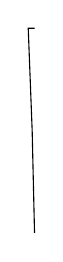
\begin{tikzpicture}[x=1cm,y=1cm]\draw (0.08,2.6)--(0,2.6)--(0.05,1.3)--(0.08,0);\end{tikzpicture}}}
\margin{\unsure{Après cela} \unsure{faire aux} \unsure{coroll. les} \unsure{corrections} \unsure{plus haut}}

\uline{Dém. \deleted{du} corollaire} Il suffit de montrer que si $\tau:\Delta_{n'}\unsure{\longrightarrow|-}\Delta_n$, d'où
\[
\mathcal A_*(\tau):\mathcal A_n\unsure{\longrightarrow|-}\mathcal A_{n'},
\]
\[
\varphi_{n'}\mathcal A_*(\tau)=\mathcal A_*(\tau)\varphi_n.
\]
\inserted{C'est clair si $n=0$ car $\mathcal A_0=S$, et par hyp. si $n=1$. Si \unsure{on a} $n\ge1$}
\margin{\unsure{Alors} \unsure{en rien}}
On regarde les $\sigma:\Delta_n\longrightarrow\Delta_1$ \deleted{\unsure{par récurrence}} (on peut se \inserted{\unsure{on n'a pas}} borner aux surjectifs) les $\mathcal A_*(\sigma):\mathcal A_1\to\mathcal A_n$ ont des images qui \uuline{engendrent} l'algèbre $\mathcal A_n$, donc il suffit de prouver que
\margin{193}

\scanpage{195}
\begin{center}- \mspage{60} -\end{center}
\margin{IX}

\uline{i.e.} \uline{définit un isomorphisme de chacun de ces schémas abéliens avec le dual de l'autre}.

La démonstration de 5.4 dans le cas général va être donnée au n° 7, comme conséquence d'une construction fort naturelle et importante due à RAYNAUD. Notons seulement ici que pour prouver 5.4, on peut supposer $S$ complet, compte tenu de 3.3.

5.5. Pour exprimer commodément les facteurs extrêmes dans les filtrations (5.1.10) et (5.1.11), dans le cas de la réduction semi-stable, introduisons les schémas en groupes constants tordus sur $S$
\[
(5.5.1)\qquad\underline M'_{\unsure{o|0}}=D(T_{\unsure{o|0}})\quad,\quad\underline M_{\unsure{o|0}}=D(T'_{\unsure{o|0}})\quad,
\]
duals des tores maximaux $T_{\unsure{o|0}},T'_{\unsure{o|0}}$ des fibres spéciales de $A,A'$ (SGA 3 X 5.7). Comme $S$ est local complet, ces schémas en groupes peuvent être considérés comme les fibres spéciales de schémas constants tordus
\[
(5.5.2)\qquad\underline M'\ ,\ \underline M\text{ sur }S\quad;
\]
ainsi, si le tore $T_{\unsure{o|0}}$ est déployé (par exemple si $k$ est séparablement clos) i.e. si $\underline M'_{\unsure{o|0}}$ est le groupe constant défini par le groupe ordinaire
\[
(5.5.3)\qquad M'=\operatorname{Hom}_{k\text{-gr}}(T_{\unsure{o|0}},\mathbb G_{mk})\quad,
\]
alors $\underline M'$ est le groupe constant défini par $M'$ :
\[
\underline M'=M'_S\quad.
\]
On peut d'ailleurs noter que, puisque $T_{\unsure{o|0}}$ et $T'_{\unsure{o|0}}$ sont isogènes (2.2.6), $T'_{\unsure{o|0}}$ est déployé si $T_{\unsure{o|0}}$ l'est, de sorte qu'il y a lieu d'introduire également
\margin{378}
\margin{378}
\margin{194}

\scanpage{196}
\[
\underbrace{\varphi_{n'}\underbrace{\mathcal A_*(\tau)\mathcal A_*(\sigma)}_{\mathcal A_*(\sigma\tau)}}_{\mathcal A_*(\sigma\tau)\varphi\ (\text{par hyp. sur }\varphi_{n'})}
=
\underbrace{\mathcal A_*(\tau)\underbrace{\varphi_n\mathcal A_*(\sigma)}_{\mathcal A_*(\sigma)\varphi\ (\text{par hyp. sur }\varphi_n)}}_{\mathcal A_*(\sigma\tau)\varphi}
\qquad\forall\sigma:\Delta_n\to\Delta_1
\]
OK.

\uline{Dém. de la prop} Le cas $n=0$ est \unsure{triv.}, pour le cas $n=1$ il faut considérer les trois cas $\sigma=\mathrm{id}$ qui donne $\varphi_1=\varphi$, puis $\sigma$ application constante de valeur $0$ ($\alpha_0$) ou $1$ ($\beta_0$), de sorte que $\mathcal A_*(\alpha_0)=\alpha$, $\mathcal A_*(\beta_0)=\beta$, et le fait que $\varphi_1=\varphi$ y soit \unsure{compatible} n'est autre que l'hyp. suppl. sur $\varphi$ sur les augmentations \inserted{$\alpha,\beta$}. On peut donc supposer $n\ge2$. Considérons les applications \inserted{croiss} $\sigma:\Delta_n\to\Delta_1$; elles sont surj. ou constantes. Considérons les surjectives, il y en a $n$, soit $\sigma_{\unsure{r}}$ ($0\le r\le n-1$)
\[
\sigma_r(0)=0,\ -\ \sigma_r(r)=0,\ \sigma_r(r+1)=1,\ -\ \sigma_r(n)=1
\]
donc \deleted{$\unsure{\mathcal A}$}
\[
\begin{cases}
\mathcal A_*(\sigma_r)(X_0)=X_0+-+X_r\overset{\mathrm{dfn}}=U_r\\
\mathcal A_*(\sigma_r)(X_1)=X_{r+1}\ -+X_n
\end{cases}
\]
On doit donc avoir
\[
\mathcal A_*(\sigma_r)(X_0^{(i)})=U_r^{(i)}
\]
\uline{Lemme} Les $U_r^{(i)}$ (\deleted{$\unsure{i}$} $i\ge1$, $0\le r\le n-1$) engendrent la \inserted{$S$-}algèbre $\mathcal A_n^0$, qui est isomorphe en fait à $\unsure{S}\{U_0,-,U_{n-1}\}$,
\margin{195}

\scanpage{197}
\begin{center}- \mspage{59} -\end{center}
\margin{IX}

désignant respectivement les parties abéliennes de $A_{\unsure{o|0}}^{\unsure{0|o}}$ et $A'_{\unsure{o|0}}{}^{\unsure{0|o}}$. Comme, en vertu de VIII 4.8, la biextension $W_{\unsure{o|0}}$ provient d'une biextension $W_{\unsure{o|0}}^{\mathrm{ab}}$ de $(B_{\unsure{o|0}},B'_{\unsure{o|0}})$ par $\mathbb G_{mk}$, déterminée à isomorphisme unique près, l'accouplement (5.3.5) peut aussi s'interpréter comme déduit de la correspondance divisorielle $W_{\unsure{o|0}}^{\mathrm{ab}}$, et l'homomorphisme correspondant
\[
(5.3.6)\qquad T_\ell(B_{\unsure{o|0}})\longrightarrow D(T_\ell(B'_{\unsure{o|0}}))\simeq T_\ell(D(B'_{\unsure{o|0}}))
\]
(où dans le dernier terme, la lettre $D$ désigne le schéma abélien dual) n'est autre que celui déduit par fonctorialité de $T_\ell$ de l'homomorphisme
\[
(5.3.7)\qquad B_{\unsure{o|0}}\longrightarrow D(B'_{\unsure{o|0}})
\]
défini par $W_{\unsure{o|0}}^{\mathrm{ab}}$. Donc le fait que (5.3.5) soit une dualité parfaite signifie aussi, par le dictionnaire bien connu (cf. [ 5]) que le noyau de (5.3.7), qui est un groupe fini sur $k$ en vertu de 1.5, a une composante $\ell$-primaire nulle. Dire qu'il en est ainsi pour tout $\ell$ signifie donc que l'isogénie (5.3.7) est un isomorphisme, i.e. que la correspondance divisorielle $W_{\unsure{o|0}}^{\mathrm{ab}}$ est une dualité parfaite entre $B_{\unsure{o|0}}$ et $B'_{\unsure{o|0}}$. Les considérations qui précédaient montrent seulement que le noyau de (5.3.7) est un $p$-groupe. Enonçons donc le résultat plus complet :

\uline{Théorème} 5.4. \uline{Soit} $S$ \uline{un trait}, \uline{et} $A_K$ \uline{un schéma abélien sur} $S$ \uline{ayant une réduction semi-stable sur} $S$. \uline{Désignons par} $B_{\unsure{o|0}},B'_{\unsure{o|0}}$ \uline{les parties abéliennes des modèles de Néron de} $A_K$ \uline{et du schéma abélien dual} $A'_K$ \uline{respectivement}. \uline{Alors la correspondance divisorielle canonique} $W_{\unsure{o|0}}^{\mathrm{ab}}$ \uline{sur} $(B_{\unsure{o|0}},B'_{\unsure{o|0}})$, \uline{déduite par} VIII 4.8 \uline{de la biextension canonique} $W_{\unsure{o|0}}$ \uline{de} $(A_{\unsure{o|0}}^{\unsure{0|o}},A'_{\unsure{o|0}}{}^{\unsure{0|o}})$ (\uline{fibre spéciale de la biextension} $W$ \uline{de} 1.4), \uline{est une dualité parfaite entre} $B_{\unsure{o|0}}$ \uline{et} $B'_{\unsure{o|0}}$,
\margin{377}
\margin{377}
\margin{196}

\scanpage{198}
\deleted{\unsure{donc}} (donc la \inserted{$S$-}algèbre engendrée par les
\[
U_{r,i}=U_r^{(i)}\qquad0\le r\le n-1,\quad i\ge1,
\]
soumis aux relations $U_{r,i}U_{r,j}=c_{ij}U_{r,i+j}$). \unsure{Et} $\unsure{=}$
\inserted{i.e. $\mathcal A_n\simeq S\{U_0,-,U_{n-1}\}[dU_0,-,dU_{n-1}]$}

C'est immédiat, car $X_0,-,X_{n-1}$ se \unsure{reconstituent} par $U_0,-,U_{n-1}$ par
\[
X_0=U_0,\ X_1=U_1-U_0,\ --,\ X_{n-1}=U_{n-1}-U_{n-2}
\]
et on a $\mathcal A_n^0\simeq S\{X_0,-,X_{n-1}\}$. \unsure{Or}

Ceci montre l'unicité de $\varphi_n$, et qu'on devra avoir
\[
\begin{aligned}
\varphi_n(\underbrace{U_{r,i}^{\deleted{\unsure{(i)}}}}_{U_r^{(i)}})
&=\varphi_n(\underbrace{\sigma_r^*}_{\substack{\Vert\,\mathrm{dfn}\\\mathcal A_*(\sigma_r)}}(X_0^{(i)}))
=\sigma_r^*(\varphi(X_0^{(i)}))\\
&=\sigma_r^*(\unsure{\xi_j|\xi_i}).
\end{aligned}
\]
i.e.
\[
\varphi_n(U_r^{(i)}\deleted{\unsure{,i}})=\sigma_r^*(\xi_i)=\deleted{\unsure{\xi_iU}}
\inserted{\left(\sum_j a_{ij}U_r^{(j)}+\left(\sum_j b_{ij}U_r^{(j)}\right)dU_r\right)}
\]
Il y a \inserted{donc} un hom. d'algèbres \inserted{unique} $\mathcal A_n^0\overset{\varphi_n^0}{\unsure{-|\longrightarrow}}\mathcal A_n$ tel que
\[
\varphi_n^0(U_r^{(i)})=\sigma_r^*(\xi_i)\overset{\mathrm{dfn}}=\xi_{r,i}
\]
car cela revient à vérifier les relations
\deleted{$\sigma_r^*(\xi_i)\sigma_r^*(\unsure{\xi_j})$}
\[
\xi_{r,i}\xi_{r,j}=c_{ij}\xi_{r,i+j}
\]
i.e.
\[
\sigma_r^*(\xi_i)\sigma_r^*(\xi_j)=c_{ij}\sigma_r^*(\xi_{i+j})
\]
\[
\Vert\qquad\sigma_r^*(\xi_i\xi_j)
\]
\[
\sigma_r^*(c_{ij}\xi_{i+j})=c_{ij}\sigma_r^*(\xi_{i+j})\qquad\text{OK}
\]
\margin{197}

\scanpage{199}
\begin{center}- \mspage{58} -\end{center}
\margin{IX}

qui est une \uline{dualité parfaite}, i.e. identifiant chacun des deux facteurs du premier membre au dual de l'autre (au sens de 5.2.2). (NB les exposants ab désignent les ``parties abéliennes'', quotient de la partie fixe par la partie torique). Il est clair d'autre part que (5.3.2) est induit par l'accouplement
\[
(5.3.3)\qquad T_\ell(A^{\unsure{0|o}})^{\mathrm{ab}}\times T_\ell(A'^{\unsure{0|o}})^{\mathrm{ab}}\longrightarrow T_\ell(\mathbb G_{mS})
\]
déduit par passages aux quotients de l'accouplement (5.2.4.2). Celui-ci étant une dualité parfaite sur les fibres génériques, i.e. l'homomorphisme correspondant
\[
(5.3.4)\qquad T_\ell(A^{\unsure{0|o}})^{\mathrm{ab}}\longrightarrow D(T_\ell(A'^{\unsure{0|o}})^{\mathrm{ab}})
\]
étant un isomorphisme sur les fibres génériques, nous avons évidemment envie d'en déduire qu'il en est de même sur $S$ tout entier, ou ce qui revient au même, sur les fibres spéciales. Cette déduction est valable, trivialement, si $\ell\ne p$ ; elle est valable également, du moins dans le cas d'inégales caractéristiques, si $\ell=p$, grâce à un théorème profond de TATE [33, th.4]. Nous allons cependant pouvoir l'établir directement, sans l'aide du théorème de Tate, plus bas (7.4.6).

Pour préciser la signification géométrique du résultat que nous désirons établir, notons que l'accouplement déduit de (5.3.3) par passage aux fibres spéciales n'est autre que l'accouplement
\[
(5.3.5)\qquad T_\ell(B_{\unsure{o|0}})\times T_\ell(B'_{\unsure{o|0}})\longrightarrow T_\ell(\mathbb G_{mk})
\]
déduit de la biextension $W_{\unsure{o|0}}$ de $(A_{\unsure{o|0}}^{\unsure{0|o}},A'_{\unsure{o|0}}{}^{\unsure{0|o}})$ par passage au quotient, $B_{\unsure{o|0}}$ et $B'_{\unsure{o|0}}$
\margin{376}
\margin{376}
\margin{198}

\scanpage{200}
Si on veut étendre $\varphi_n^0$ en \deleted{$\unsure{\varphi}$} hom de $S$-algèbre $\varphi_n:\mathcal A_n-\mathcal A_n$, il faut se donner les images des $dU_0,-,dU_{n-1}$, et vérifier seulement que ce sont des éléments de \uline{carré nul}, \deleted{\unsure{et réciproquement}} \inserted{qui \uline{anticommutent entre eux} et commutent aux $\xi_{s,i}$}.
\[
\varphi_n(dU_r)=d\varphi_n(U_r)=d\sigma_r^*(\xi_1)=\sigma_r^*(d\xi_1)
\]
\[
\left(=d\left(\sum_{j\geq0}a_{1j}U_r^{(j)}\right)
=\left(\sum_{j\geq1}a_{1j}U_r^{(j-1)}\right)dU_r\right)
\]
\margin{$d\xi_1=\sum_{j\geq1}a_{1j}X_0^{(j-1)}dX_0$
\deleted{$d\xi_1=\sum_{j\geq1}a_{1j}X_0^{(j-1)}dX_0$}}
Ces éléments sont bien de carré nul, anticommutent entre eux, mais commutent-ils aux
\[
\xi_{s,i}=\sigma_s^*(\unsure{\varphi(X_0^{(i)})|X_0^{(i)}})
=\sum_{j\geq0}a_{ij}U_s^{(j)}+\left(\sum_{j\geq0}b_{ij}U_s^{(j)}\right)dU_s
\]
\deleted{\unsure{en résumé}, \unsure{précisément}
\[
\mathcal A_n=S\{U_0,-,U_{n-1}\}[dU_0,-,dU_{n-1}]
\]
et \unsure{pour $\xi$ on a}
\[
F+\sum_{0\leq r\leq n-1}G_r\,dU_r
\]}
\margin{et $\sigma_r^*(d\xi_1)$ commute bien aux $\xi_{s,i}=\sigma_s^*(X_0^{(i)})$ pour $s=r$, mais pour $s\neq r$ c'est vrai ssi
\[
2\left(\sum_{j\geq1}a_{1j}U_r^{(j-1)}\right)\left(\sum_{j\geq0}b_{ij}U_s^{(j)}\right)=0,
\]
i.e.
\[
\boxed{2a_{1j}b_{ik}=0\quad\forall\uline{$j\geq1$},\ k\geq0}.
\]
Or $a_{11}=1+\sum_{i\geq\unsure{1}}\alpha_i T^{(i)}$ est \unsure{un div. $\not\!$ zéro|non div. de zéro}, donc il faut
\[
2b_{ik}=0\quad\forall i\geq1,\ k\geq0
\]
donc $2B_i=0$.}
On utilise, pour prouver que $\varphi_n$ (qui à priori est un endom de $S$-algèbres) commute à la différentielle, on utilise le

\uline{Lemme} $S$ un anneau commutatif, $U_0- U_m$ des variables, on considère \deleted{\unsure{Alors}} la $S$-algèbre diff $A=S\{U_0,-,U_m\}[dU_0,-,dU_m]$
(\uline{NB} on néglige la structure des p.d., \unsure{mais on a} $dU_r^{(i)}=U_r^{(i-1)}dU_r-$).
Soit $B$ une $S$-alg. diff. \unsure{alternée}, (gr.d. mod $2$, différentielle de degré $1$),
On s'intéresse aux hom d'algèbres diff. $A\xrightarrow{\varphi}B$. Pour tt tel, on
\margin{199}

\scanpage{201}
\hfill -- \mspage{57} -- \hfill IX

5.2.6. Supposons maintenant que $A_K$ ait une réduction semi-stable sur $S$, de sorte que nous pouvons prendre pour $\ell$ n'importe quel nombre premier (distinct ou non de $p$). D'ailleurs, en vertu du critère galoisien de réduction semi-stable 3.5, on a pour $\ell\neq p$
\[
\text{(5.2.7)}\qquad (T_\ell(A'_K)^f)^\perp\quad (=T_\ell(A_K)^t)\subset T_\ell(A_K)^f\quad .
\]
Il reste à prouver, pour terminer la preuve de 5.2, que cette inclusion est valable sans restriction sur $\ell$.

En effet, le membre de gauche est canoniquement isomorphe à $D(T_\ell(A'_K)/T_\ell(A'_K)^f)$, et est donc de ``rang'' (ou ``hauteur'') égal à $2n-2\alpha-\mu=\mu$ (notations de (2.1.9), où par hypothèse $\lambda=0$), qui est aussi celui de $T_\ell(A_K)^t$. Comme l'inclusion
\[
\text{(*)}\qquad T_\ell(A_K)^t\subset T_\ell(A_K)
\]
est \uline{stricte}, dans le sens qu'elle induit déjà un monomorphisme pour tous les termes du systèmes projectifs envisagés, il s'ensuit aisément que le premier membre de (*) est maximal parmi les sous-pro-groupes de Barsotti-Tate de $T_\ell(A_K)$ ayant même rang que lui, de sorte qu'on a bien l'égalité de (5.2.7), qui équivaut à l'inclusion entre les termes extrêmes de 5.2.7 par le théorème d'orthogonalité.

5.3. Utilisant la correspondance par orthogonalité entre sous-pro-groupes de Barsotti-Tate stricts (au sens précisé plus haut) des pro-groupes duaux $T_\ell(A_K)$ et $T_\ell(A'_K)$, on déduit formellement de (5.2.2) que l'accouplement (1.0.2) entre ces pro-groupes induit un accouplement
\[
\text{(5.3.2)}\qquad T_\ell(A_K)^{ab}\times T_\ell(A'_K)^{ab}\longrightarrow T_\ell(\mathbf G_{mK})
\]
\margin{375}
\margin{375}
\margin{200}

\scanpage{202}
\[
X_0+\underbrace{\sum_{i,j\geq1}f_{ij}X_0^{(i)}\sum_{0\leq k\leq j}T^{(j-k)}(-1)^kX_0^k}_{\displaystyle\sum_{\substack{i,j,k\\0\leq k\leq j;\ i,j\geq1}}f_{ij}T^{(j-k)}(-1)^kX_0^{i+k}}
\]
\[
\deleted{=\sum}\qquad
\left\{\begin{array}{l}
\underline{i+k}=\text{\textcircled{$\nu$}}\geq1\\
0\leq\text{\textcircled{$k$}}\leq\nu-1\\
j\geq\operatorname{Sup}(k,1)
\end{array}\right.
\qquad
\begin{array}{l}
i=\nu-k\geq1\\
j=k+\delta\quad\delta=j-k\\
\delta\geq0
\end{array}
\]
\[
\deleted{\sum_\nu X_0^\nu\sum_{\substack{0\leq k\leq\nu-1\\\deleted{j\geq\operatorname{Sup}(k,1)}\\\inserted{\delta\geq0}\\\inserted{(k,\delta)\neq(0,0)}}}(-1)^k f_{\unsure{i},k+\delta}T^{\deleted{\unsure{(j-k)}}\inserted{\delta}}}
\]
\[
\sum_{\nu\geq1}X_0^\nu\underbrace{\sum_{\substack{0\leq k\leq\nu-1\\\delta\geq0\\\deleted{(k,\delta)\neq0}\\\inserted{k+\delta\geq1}}}(-1)^k f_{\nu-k,k+\delta}T^\delta}_{a_{1,\nu}}
\]
\deleted{$\unsure{=}$}
\[
A_0=X_0\overbrace{\left(1+\sum_{\delta\geq1}f_{1,\delta}T^{(\delta)}\right)}^{a_{1,1}}+\sum
\]
\[
(k=0,\nu=1)
\]
\figure{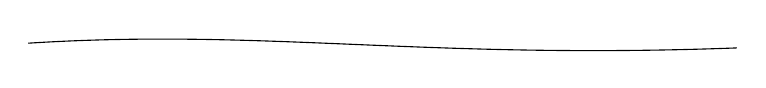
\begin{tikzpicture}\draw (0,0.06) .. controls (3,0.25) and (5,-0.15) .. (9,0);\end{tikzpicture}}
\[
\unsure{\varphi(\xi_1}\qquad\varphi(X_0)
\]
\margin{201}

\scanpage{203}
\margin{202}
\hfill -- \mspage{56} -- \hfill IX

\uline{Lemme} 5.2.5. \uline{Soit} $u:G\longrightarrow H$ \uline{un homomorphisme de pro-$\ell$-groupes de Barsotti-Tate sur} $S$. \uline{Si} $u_o:G_o\longrightarrow H_o$ \uline{est nul}, \uline{alors} $u$ \uline{est nul}. \uline{Si} $u_o:G_o\longrightarrow H_o$ \uline{est une isogénie} (resp. \uline{un isomorphisme}), $u$ \uline{est une isogénie} (resp. \uline{un isomorphisme}).

Nous appliquerons en effet la première assertion de 5.2.5 au morphisme composé
\[
T_\ell(A^{\unsure{0|o}})^t\longrightarrow T_\ell(A^{\unsure{0|o}})^f\longrightarrow D(T_\ell(A'^{\unsure{0|o}})^f)\quad ,
\]
où le deuxième morphisme est celui déduit de l'accouplement (5.2.4.2), on trouve que ce composé est nul, donc que l'accouplement envisagé s'annule sur la partie torique à gauche. Par symétrie, il s'annule donc sur la partie torique à droite, donc il provient d'un accouplement sur les quotients, ou ``morceaux abéliens''
\[
T_\ell(A^{\unsure{0|o}})^{ab}\times T_\ell(A'^{\unsure{0|o}})^{ab}\longrightarrow T_\ell(\mathbf G_m)\quad ,
\]
lesquels quotients sont encore des pro-groupes de Barsotti-Tate, comme on vérifie aisément. Il reste à prouver que le morphisme correspondant à cet accouplement
\[
T_\ell(A^{\unsure{0|o}})^{ab}\longrightarrow D(T_\ell(A'^{\unsure{0|o}})^{ab})
\]
est une isogénie, ce qui résulte encore de 5.2.5.

Nous laisserons au lecteur la démonstration (facile) de 5.2.5, qui est un résultat valable sur toute base noethérienne connexe. Nous trouverons d'ailleurs plus bas (7.4.7), par une analyse un peu plus précise des biextensions $W_n$ des $(A_n^{\unsure{0|o}},A_n'^{\unsure{0|o}})$, une démonstration directe assez évidente des deux cas particuliers où nous avons eu à utiliser 5.2.5.
\margin{374}
\margin{374}

\scanpage{204}
Endomorphismes de l'anneau différentiel $\frac12$ simplicial $\mathcal A_*$

(NB. on ne demande plus de respecter la structure de $S$-algèbre, $S=\mathcal A_0$, i.e. on ne demande plus que $\varphi_*$ induise l'identité sur $\mathcal A_0$).

Rappelons-nous qu'un complexe de De Rham peut se construire \unsure{dès que l'on a} un anneau comm. $S$ avec idéal $S^+$ à puiss. divisées, et $t\in S^+$, i.e. une \deleted{\unsure{algèbre}} \inserted{$S$-algèbre} différentielle \inserted{$\mathbb N$-graduée, à p.d.} $\frac12$ simpliciale $\mathcal A_*(S,S^+,t)$, où
\[
\mathcal A_n(S,S^+,t)=S\{X_0,-,X_n\}[dX_0,-,dX_n]/\bigl(\sum X_i-t,\ \sum dX_i\bigr)_{pd}
\]
Si on a un hom. d'anneaux à p.d.
\[
S\xrightarrow{u}S'\quad(u(S^+)\subset S'^+-)\quad\text{et}\quad\lambda'\in S'
\]
tel que \deleted{$\unsure{\lambda\in S'^+}$} $u(t)=\lambda t'$, on définit un hom \inserted{de $S$-\unsure{alg. $\mathbb N$-graduées} différentielles à p.d.}
\[
\mathcal A_*(u,\lambda):\mathcal A_*(S,S^+,t)-\mathcal A_*(S',S'^+,t'),
\]
qui en degré $n$ est l'hom.
\diagram{\begin{tikzcd}
S\{X_0,-,X_n\}[dX_0,-,dX_n]/-\arrow[d]\\
S'\{X_0,-,X_n\}[dX_0,-,dX_n]/-
\end{tikzcd}}
donné par \deleted{$\unsure{X_0\longmapsto}$} $u:S-S'$ sur les scalaires,
\[
X_0\longmapsto\lambda X_0\quad\left(\text{donc }\sum X_0-t\longmapsto\sum\lambda X_0-u(t)=\sum\lambda X_0-\lambda t'=\lambda(\sum X_0-t')\right)
\]
$dX_0\longmapsto\lambda dX_0$. Ainsi $\mathcal A_*(S,S^+,t)$ devient un foncteur covariant de la catégorie des triples $(S,S^+,t)$, où les hom sont les couples $(u,\lambda)$ \inserted{\fbox{comme dessus}} (\unsure{composés} par $(u',\lambda')(u,\lambda)=(u'u,u'(\lambda)\lambda')$).

\uline{NB} En plus de sa graduation, $\mathcal A_n(S,S^+,t)$ admet une filtration \inserted{croissante} naturelle, où $\operatorname{Fil}^{\unsure{n}}\mathcal A_n(S,S^+,t)$ est la somme des expressions
\[
\sum F_{i_0- i_p}\,dX_{i_0}\wedge-\wedge dX_{i_p},
\]
avec $F_{i_0-i_p}\in S\{X_0,-,X_n\}$ étant de ``degré'' $\leq\unsure{n-r|n-p}$, ce sont des sous-$S$ modules (mais pas des idéaux), on a
\[
\operatorname{Fil}^n.\operatorname{Fil}^m\subset\operatorname{Fil}^{n+m},\quad\operatorname{Fil}^0=S\ (\text{scalaires}),\quad\operatorname{Fil}^n=0\text{ si }n<0.
\]
Cette filtration est respectée par les $\mathcal A_*(u,\lambda)$.
\margin{203}

\scanpage{205}
\hfill -- \mspage{67} -- \hfill IX

En effet, la dernière hypothèse faite nous ramène au cas où $G'=A$, $u=\text{identité}$, et où $v_\eta:G_\eta\longrightarrow A_\eta$ est donc une projection, qu'on se propose de prolonger en une projection $v:G\longrightarrow A$. Or $G$ est \uline{lisse} comme extension de deux schémas en groupes lisses, de sorte que la conclusion résulte de la définition de la propriété néronienne de $A$.

\uline{Corollaire} 5.10. \uline{Soient} $A_K$ \uline{un schéma abélien sur le corps des fonctions} $K$ \uline{d'un trait} $S$, $\ell$ \uline{un nombre premier}. \uline{Lorsque} $\ell=p$, \uline{on suppose} $\operatorname{car}.K=0$, \uline{pour pouvoir disposer du théorème de TATE déjà invoqué dans} 5.8. \uline{Pour que} $A_K$ \uline{ait bonne réduction sur} $S$, \uline{il faut et il suffit que le pro-$\ell$-groupe de Barsotti-Tate} $T_\ell(A_K)$ ``\uline{ait bonne réduction sur} $S$'', \uline{i.e.} \uline{se prolonge en un groupe de Barsotti-Tate sur} $S$.

(C'est le résultat conjecturé dans [8, 4.9].)

La nécessité étant claire, il reste à prouver la suffisance ; notons d'ailleurs que le cas $\ell\neq p$ a déjà été traité (2.2.9). On peut supposer $S$ hensélien (2.2.9). Supposons d'abord que $A_K$ ait réduction semi-stable sur $S$. Alors 5.8 appliqué à $F=X$ nous montre qu'on a $T_\ell(A_K)=T_\ell(A_K)^f$, ce qui signifie aussi que le tore maximal de $A_o$ est nul, i.e. que $A_o^{\unsure{0|o}}$ est un schéma abélien, de sorte que la conclusion résulte de (2.2.9 (iii$^\circ$)). Traitons maintenant le cas général. En vertu de 2.2.9 on peut supposer évidemment $S$ strictement local. Soir $K'$ une extension galoisienne finie telle que $A_{K'}$ ait réduction semi-stable sur le normalisé $S'$ de $S$ dans $K'$ (3.6). Si $A^*$ désigne le modèle de Néron correspondant, $G=\operatorname{Gal}(K'/K)$ opère sur la situation $(A^*,S')$, donc sur
\margin{385}
\margin{385}
\margin{204}

\scanpage{206}
Considérons le cas où $t'\in S'^+$ est un élément régulier de $S'$; alors $\lambda$ tel que $u(t)=\lambda t'$ est uniquement déterminé par $u$; donc si on se borne aux triples $(S,S^+_{p.d.},t)$ tels que $t$ soit régulier, et aux hom $u:(S,S^+\deleted{,t})\longrightarrow(S',S'^+\deleted{,t'})$ tels que $u(t)\in S.t'$, alors $\mathcal A_*(S,S^+,t)$ devient un foncteur sur cette catégorie, à valeurs ds la cat. des \deleted{\unsure{des}} anneaux gradués \inserted{(\unsure{alternés})} \deleted{\unsure{et}} différentiels filtrés.

La condition envisagée sur $(S,S^+_{pd},t)$ est vérifiée en particulier si on fait $S=k\{T\}$, $S^+=(T)_{pd}$, $t=T$, lorsque $k$ est sans torsion.

Revenons donc à
\[
\mathcal A_*(k)\overset{\mathrm{dfn}}=\mathcal A_*(\underset{k\{T\}}{S_k},S_k^+,T),
\]
et à la détermination des endom de $\mathcal A_*(k)$, comme \deleted{\unsure{anneaux}} \inserted{$k$-algèbre} différentielle $\frac12$ simpliciale (où on ne considère \deleted{\unsure{pas}} la structure de $S$-algèbre, ni la graduation ni les p.d., ni sa filtration a priori-). \deleted{\unsure{Bien à ce propos où}}
Soit $G_k$ le \deleted{groupe} \inserted{monoïde} des couples $(u,\lambda)$, où $u$ est un endom. de $S$ comme $k$-algèbre à p. div., et $\lambda\in S^{\deleted{\unsure{*|+}}}$ tel que $u(T)=\lambda\{T\}T$. Comme $u\deleted{\unsure{(T)}}$ est connu par la connaissance de $u(T)$, $G_k$ est donc le \deleted{groupe} \inserted{monoïde} \unsure{d'ens. sous-jacent} $S$, avec la multiplication
\[
(\lambda'*\lambda)\{T\}\deleted{\unsure{*}}=\lambda'\{T\}\lambda\{T\lambda'\{T\}\}
\]
\deleted{\unsure{de $S^\times$}} --- on désigne par $(u_\lambda)_*$ l'endomorphisme de $\mathcal A_*(k)$ défini par $\lambda\in S$ (et $u_\lambda u_{\lambda'}=u_{\lambda\lambda'}$).
Il est clair que $\lambda\longmapsto u_{\lambda*}$ est un hom de monoïdes \uline{injectif} (en fait $\lambda\longmapsto(u_\lambda)_1$ l'est déjà, car $(u_\lambda)_*(X_0)=\lambda X_0$ et $\mathcal A_1(k)\simeq k\{T\}\{X_0\}$.
Ceci dit,

Si $H_k$ est le monoïde des $\unsure{S_k|G_k}$-endomorphismes de la $k$-algèbre différentielle $\frac12$ simpliciale $\mathcal A_*(k)$, \deleted{et} \deleted{\unsure{est que}} $\Omega_k$ le monoïde de \uline{tous} les endomorphismes de la $k$-alg. diff. $\frac12$ simpliciale, on a
\margin{205}

\scanpage{207}
\hfill -- \mspage{52} -- \hfill IX

Comme le foncteur $X\longmapsto\widehat X$ (complétion formelle le long de la fibre spéciale) induit une équivalence entre la catégorie des schémas finis sur $S$, et celle des schémas formels finis sur $S$ (EGA III 4.8), nous allons identifier simplement un schéma fini sur $S$ avec le schéma formel correspondant. Avec cette identification, la définition des ``parties fixes'' nous donne aussitôt pour tout $\nu\geq0$ :
\[
\text{(5.1.4)}\qquad ({}_{\ell^\nu}A^{\unsure{0|o}})^f={}_{\ell^\nu}(\widehat A^{\unsure{0|o}})\quad ,
\]
ce qu'on peut écrire aussi comme une identité de systèmes projectifs
\[
\text{(5.1.5)}\qquad T_\ell(A^{\unsure{0|o}})^f=T_\ell(\widehat A^{\unsure{0|o}})\quad .
\]
On obtient donc un sous-pro-groupe de Barsotti-Tate de la partie fixe de $T_\ell(A^{\unsure{0|o}})$ en prenant $T_\ell(\widehat T)\subset T_\ell(\widehat A^{\unsure{0|o}})$. On définira alors la \uline{partie torique} de $T_\ell(A^{\unsure{0|o}})$ comme
\[
\text{(5.1.6)}\qquad T_\ell(A^{\unsure{0|o}})^t\overset{\mathrm{dfn}}=T_\ell(\widehat T)\subset T_\ell(\widehat A^{\unsure{0|o}})=T_\ell(A^{\unsure{0|o}})^f\quad .
\]
Donc par définition, on aura
\[
\text{(5.1.7)}\qquad T_\ell(A^{\unsure{0|o}})^t=({}_{\ell^\nu}\widehat T)_{\nu\geq0}\quad ,
\]
le $S$-groupe fini et plat ${}_{\ell^\nu}\widehat T$ étant lui-même décrit comme la limite inductive des $S_n$-groupes finis et plats
\[
\text{(5.1.8)}\qquad {}_{\ell^\nu}(T_n),\ n\text{ variable}\quad ,
\]
i.e. son algèbre affine est décrite comme la limite projective des algèbres affines des groupes (5.1.8). Bien entendu, on aura
\[
\text{(5.1.9)}\qquad (T_\ell(A^{\unsure{0|o}})^t)_n=T_\ell(T_n)\quad ,
\]
\margin{370}
\margin{370}
\margin{206}

\scanpage{208}
\[
G_k,H_k\subset\Omega_k
\]
\[
G_k\cap H_k=\{u_\lambda\mid\lambda\in S_k,\ \lambda T=T\ \text{i.e. }(\lambda\{T\}-1)T=0\}
\]
Si on pose $\lambda\{T\}=\sum_{i\geq0}\lambda_i T^{(i)}$, alors la condition sur $\lambda$ envisagée est
\[
\boxed{\lambda_0=1}\quad\deleted{\lambda_0=1},\qquad\boxed{(i+1)\lambda_i=0\qquad\forall i\geq1}
\]
\deleted{Ce qui implique en particulier $\lambda_0=1$.}
\deleted{\unsure{$k$ de car. $0$, cela implique plus que}}
Si $k$ sans torsion, cela implique $\lambda_i=0$ pour $i\geq1$ i.e. $\lambda=1$, i.e. $u_\lambda=\operatorname{id}$, d'où $G_k\cap H_k\inserted{=\unsure{(e)|\{e\}}}$ dans ce cas, --- et dans ce cas seulement.
[Dans ce cas, \inserted{$k$ de car. $0$ i.e. une $\mathbf Q$-alg.,} $G_k$ est aussi le groupe \inserted{$G'_k$} de tous les endom. de $S_k=k\{T\}$ comme $k$-alg. \uline{augmentée} \deleted{\unsure{p.d.}} et par suite \deleted{l'hom. \unsure{dans} $\Omega$}
\diagram{\begin{tikzcd}[column sep=small]
(\unsure{1|0}\arrow[r] & H'_k\arrow[r] & )\,\Omega_k\arrow[r,dash] & G'_k=\operatorname{End}_{\substack{k\text{-alg}\\\deleted{\mathrm{aug}}}}(\underset{S_k}{\underbrace{k\{T\}}})\\
&&&G_k\arrow[u,"(??)"]\arrow[ul,bend left=28]
\end{tikzcd}}
donne $\Omega_k$ comme produit $\frac12$ direct de $G_k\inserted{\simeq G'_k}$ et de $H'_k$\unsure{\ldots} ]

\deleted{Dans le cas général, on peut dire que}
\diagram{\begin{tikzcd}[column sep=small]
1\arrow[r,dash] & H_k\arrow[r,dash] & \unsure{\Omega_k}\arrow[r] & \unsure{G'_k|G_k}=\operatorname{End}_{k\text{-alg. augm.}}(k\{T\})\\
&&&G_k\arrow[u]\arrow[ul,bend left=28]\arrow[ul,bend right=18,dash]\\
&&&G_k\cap H_k\simeq\{u_\lambda\mid\lambda=1+\sum_{i\geq1}\lambda_iT^{(i)},\ (i+1)\lambda_i=0\}\arrow[u]
\end{tikzcd}}
\margin{207}

\scanpage{209}
\margin{208}
\hfill -- \mspage{51} -- \hfill IX

5. \uline{Le théorème d'orthogonalité dans le cas} $\ell=p$ (\uline{cas semi-stable}). \uline{Dualité des schémas abéliens} $B_o$ \uline{et} $B'_o$. \uline{Caractérisation de la partie fixe}. \uline{Critères de bonne réduction}, \uline{de bonne réduction essentielle et semi-stable}.

5.1. Plaçons nous dans le cas 2.2.3 où $S$ est hensélien et $A^{\unsure{0|o}}$ est $\ell$-divisible, de sorte que la \uline{partie fixe}
\[
T_\ell(A^{\unsure{0|o}})^f\lhook\joinrel\longrightarrow T_\ell(A)
\]
est définie comme le pro-$\ell$-groupe de Barsotti-Tate formé des $({}_{\ell^\nu}A^{\unsure{0|o}})^f$.
Nous allons maintenant donner une définition de la partie torique (2.3.2) de $T_\ell(A^{\unsure{0|o}})$, indépendante de l'hypothèse $\ell\neq p$ faite dans 2.3, mais supposant en revanche $S$ \uline{complet} (*). Pour ceci, introduisons pour tout entier $n\geq0$ le schéma artinien local
\[
\text{(5.1.1)}\qquad S_n=\operatorname{Spec}(V/\underline m^{n+1})\quad ,
\]
n.ème voisinage infinitésimal de $s$ dans $S$, et pour tout $S$-schéma $X$ soit $X_n=X\times_S S_n$. Comme $(A^{\unsure{0|o}})_n=(A_n)^{\unsure{0|o}}$ est lisse sur $S_n$, il est connu (SGA 3 IX 3.6 bis) que $T_o$ est la fibre spéciale d'un unique sous-tore
\[
\text{(5.1.2)}\qquad T_n\subset A_n^{\unsure{0|o}}\quad .
\]
D'après l'unicité des $T_n$, ceux-ci se déduisent les uns des autres par les changements de base $S_{n'}\longrightarrow S_n$. En d'autres termes, il définissent un \uline{sous-tore formel} $\widehat T$ du groupe $\widehat A^{\unsure{0|o}}$ (dans la catégorie des schémas formels sur $S$) complété formel de $A^{\unsure{0|o}}$ le long de la fibre spéciale :
\[
\text{(5.1.3)}\qquad\widehat T\subset\widehat A^{\unsure{0|o}}\quad .
\]
\margin{(*) Cette hypothèse n'est d'ailleurs pas essentielle, comme on montre dans 6.1 ci-dessous.}
\margin{369}
\margin{369}

\scanpage{210}
Essayons de déterminer directement les $\varphi_*$, endom de la $k$-alg. diff. $\frac12$ simpliciale $\mathcal A_*(k)$.

1) Premier invariant $\varphi_0\in\operatorname{End}_{k\text{-alg}}(S_k)$.
\deleted{$\varphi_0$} $\varphi_0$ est donné par les
\[
\varphi_0(\unsure{T^i|T^{(i)}})=\text{\textcircled{$\tau_i$}}\in S_k\qquad i\geq1
\]
satisfaisant les conditions
\[
\boxed{\tau_i\tau_j=c_{ij}\tau_{i+j}}
\]
Chaque $\varphi_n$ est $\varphi_0$-semi-linéaire.

2) \uline{Deuxième} invariant $\varphi_1$, endom $\varphi_0$-semi-linéaire de $S_k\{X_0\}[dX_0]$, considéré comme $S_k$-alg. différentielle (\unsure{sans sa|plus sa} graduation avec prop. anti-comm.\unsure{)}.
\inserted{Il doit être compatible avec les augm. $\alpha$ et $\beta$.}

\uline{Prop} Soit $S,S'$ deux anneaux comm., $\varphi_0:S-S'$ un hom, on s'intéresse à la détermination des homs d'anneaux différentiels
\[
\varphi_1:\underbrace{S\{X_0\}[dX_0]}_{A_S}-\underbrace{S'\{X_0\}[dX_0]}_{A_{S'}}
\]
induisant $\varphi_0$ sur $S$, et compatibles aux augmentations $(X_0\longmapsto0,dX_0\longmapsto0)$. Ils sont donnés exactement par des systèmes d'éléments
\[
\underset{\substack{\Vert\\A_i+B_i\,dX_0}}{\xi_i}\in A_{S'}^+=\operatorname{Ker}(\alpha_{S'}:A_{S'}\longrightarrow S')
\]
\[
A_i\in S\{X_0\}^+,\ B_i\in S\{X_0\}\qquad A_i=A_1^{(i)}
\]
satisfaisant :
$\varphi_1$ étant déterminé par les $\xi_i$ \unsure{via} :
\[
\varphi_1(X_0^{(i)})=\xi_i
\]
\[
\varphi_1(dX_0)=d\xi_1
\]
$\varphi$ est compatible avec les graduations (resp. les p.d.) ssi $B_i=0$ $\forall i\geq1$ (resp. $B_i=A_1^{(i-1)}B_1\quad\forall i\geq2$).
\margin{209}

\scanpage{211}
\hfill -- \mspage{50} -- \hfill IX

apparaît comme un quotient de $\mathbb Q[T]/(T^{p^N}-1)$, qui est un composé direct de corps extensions finies de $\mathbb Q$. Il en est donc de même de $E_{\mathbb Q}$. Considérant les images de $E,u,v$ dans les corps composants $K_i$ de $E_{\mathbb Q}$, on est donc ramené à voir que si $K=\mathbb Q(u)$ est un corps engendré par une racine primitive $p^n$-ème de l'unité $u$, et si $n$ est un entier $\geq2$ tel que $u-1\equiv0\ \operatorname{mod}n$ (dans l'anneau des entiers de $K$), alors on a $u=1$, ou $u=-1$ et $n=2$. Or ceci résulte aussitôt du fait bien connu que si $u\neq1$ i.e. $m\geq1$, l'idéal $(u-1)$ est premier et l'idéal $(p)$ en est une puissance, dont l'exposant est $>1$ sauf si $p=2,m=1$ i.e. si $u=-1$. Du fait que $(u-1)$ est premier et divise $p$ résulte en effet que $n\geq2$ ne peut diviser $u-1$ que si $n=p$, et $p$ ne divise $u-1$ que si $(u-1)=(p)$ i.e. $u=-1$, donc $n=2$.

4.7.4. Démontrons 4.7.2. Il suffit de prouver que $\Gamma$ est commutatif. Or si $x,y\in\Gamma$, on aura $(xy)(xy)=1$, ce qui peut s'écrire aussi, puisque $x^2=1,y^2=1$, $xy=(xy)^{-1}=y^{-1}x^{-1}=yx$, cqfd.

\uline{Remarque} 4.7.5. La démonstration donnée 4.7.3, jointe à 4.7.2, nous montrent que si $G$ est un Groupe commutatif divisible d'un Topos, $n\geq2$ un entier, et $\Gamma$ un groupe fini, opérant fidèlement sur $G$ en induisant l'identité sur ${}_nG$, alors $\Gamma$ est réduit à l'identité si $n\geq3$, et est isomorphe à un groupe $(\mathbb Z/2\mathbb Z)^r$ si $n=2$.
\margin{368}
\margin{368}
\margin{210}

\scanpage{212}
\[
\varphi_1(X_0^{(i)})=\text{\textcircled{$\xi_i,\ i\geq1$}}\qquad\boxed{\xi_i\xi_j=c_{ij}\xi_{i+j}}\quad(i,j\geq1)
\]
\[
\varphi_1(dX_0)=d\xi_1\qquad\boxed{d\xi_i=\xi_{i-1}d\xi_1}\qquad\boxed{\xi_i\in\unsure{S'}\{X_0\}^+}
\]
\[
\xi_i=A_i+B_i\,dX_0\qquad A_i,B_i\in S'\{X_0\}\qquad A_i\in S'\{X_0\}^+
\]
\[
dA_i=A_{i-1}A'_1
\]
\[
A_i=\unsure{\xi_1|A_1}^{(i)}
\]
\figure{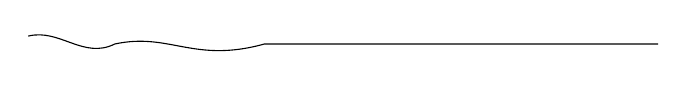
\begin{tikzpicture}\draw (0,0.1) .. controls (0.4,0.2) and (0.7,-0.2) .. (1.1,0) .. controls (1.8,0.15) and (2.1,-0.25) .. (3,0) -- (8,0);\end{tikzpicture}}
\uline{Remarque} On voit donc que tt $\varphi_1$ se met de façon \uline{unique} sous la forme $\psi_1\circ\overline\varphi_0$, où $\overline\varphi_0$ est l'hom qui prolonge $\varphi_0$ ($\overline\varphi_0(X_0^{(i)})=X_0^{(i)}$, $\overline\varphi_0(dX_0)=\deleted{\unsure{\varphi}}dX_0$) et $\psi_1$ est un $S'$-endom de la $S'$-alg. diff. $A_{S'}$, compatible avec l'augmentation.

Il faut maintenant exprimer la compatibilité de $\varphi_1$ aux augmentations $\beta$ \inserted{(si $S=k\{T\},S'=k'\{T\}$)} ($X_0\longmapsto T$, \inserted{et $X_0^{(i)}\longmapsto T^{(i)}$} $dX_0\longmapsto0$).
On trouve que l'on doit avoir
\[
\beta_{S'}(\xi_i)=\varphi_0(T^{(i)})\quad\text{i.e.}\quad\deleted{\unsure{A_{S'}}}\beta_{S'}(A_i)=\overline\varphi_0(T^{(i)})
\]
ce qui revient, puisque $A_i=A_1^{(i)}$, à
\inserted{\[
\left\{\begin{array}{l}
\beta_{S'}(A_1)=\overline\varphi_0(T)\\
\varphi_0(T^{(i)})=\varphi_0(T)^{(i)}
\end{array}\right.
\]}
donc on a
\[
A_1\deleted{\unsure{\{X_0\}}}=X_0+f\deleted{\unsure{\{X_0\}}}
\]
où $f\in\mathcal A_{\deleted{\unsure{*}}1}\simeq k\{X_0,X_1\}$ est donné par
\[
f=\sum_{i\geq1,j\geq1}X_0^{(i)}X_1^{(j)}
\]
La \uline{remarque} ci-dessus se prolonge \unsure{en}
\margin{211}

\scanpage{213}
\hfill -- \mspage{49} -- \hfill IX

On peut évidemment supposer $S$ strictement local. Avec les notations de 4.1 et de 4.2, prenons $K'$ le plus petit possible, i.e. supposons que $\Gamma$ opère \uline{fidèlement} sur $A_o^{*\unsure{0|o}}$. Par hypothèse, $\Gamma$ opère trivialement sur ${}_nA(\overline K)$, et à fortiori sur ${}_nA(\overline K)^{ef}\simeq{}_nA_o^*(k)\supset{}_nA_o^{*\unsure{0|o}}(k)$. On conclut alors par les deux lemmes suivants :

\uline{Lemme} 4.7.1. (J.P. SERRE). \uline{Soient} $G$ \uline{un schéma en groupes commutatif sur un corps} $k$, \uline{extension d'un schéma abélien par un tore}, $n$ \uline{un nombre entier} $\geq2$. \uline{Alors tout automorphisme d'ordre fini de} $G$ \uline{induisant l'identité sur} ${}_nG$ \uline{est réduit à l'identité si} $n\neq2$, \uline{et est l'identité ou d'ordre deux si} $n=2$.

\uline{Lemme} 4.7.2. \uline{Un groupe fini dont tout élément} $\neq1$ \uline{est d'ordre} $2$ \uline{est isomorphe à} $(\mathbb Z/2\mathbb Z)^r$, \uline{pour un} $r\geq0$ \uline{convenable}.

4.7.3. Rappelons la démonstration de 4.7.1, qui est bien connue. On note que grâce au fait que $n\operatorname{id}_G$ est un épimorphisme, l'hypothèse que $u$ induise l'identité sur ${}_nG$ i.e. que $1-u$ induise $0$ sur ${}_nG$, s'exprime par la condition que l'on ait $1-u=nv$ dans l'anneau des endomorphismes de $G$. Pour prouver la conclusion annoncée, on est ramené (en décomposant le groupe cyclique fini engendré par $u$ en ses composantes $p$-primaires, pour les divers nombres premiers $p$ divisant l'ordre de $u$) au cas où $u$ est d'ordre $p^N$, puissance d'un nombre premier. Soit $E$ le sous-anneau de $\operatorname{End}(G)$ engendré par $v$, qui est un quotient de $\mathbb Z[T]/(T^{p^N}-1)$, donc de type fini sur $\mathbb Z$, et qui de plus est sans torsion (ceci est conséquence formelle du fait que $G$ est divisible). Il se plonge donc dans $E_{\mathbb Q}=E\otimes_{\mathbb Z}\mathbb Q$, qui
\margin{367}
\margin{367}
\margin{212}

\scanpage{215}
\margin{\boxed{\text{p.d. dans les anneaux alternés}}}
\margin{Feuille \unsure{jaunie|paumée}...}
\uline{Théorème} Soient $S$ un anneau muni d'un idéal $I$ à puiss. divisées, $M^*=M^0+M^1$ un $S$-module gradué mod $2$,
\[
A(\unsure{M^*})=\Gamma^*(M^0)\otimes_S\Lambda^*M^1
\]
\inserted{$S$-algèbre} graduée par la parité du degré total, [et augmentée vers $S$ de la façon évidente $\varepsilon:A\longrightarrow S$] $J$ \unsure{l'idéal} engendré dans $A$ par $I$ $(\subset S\subset A)$ et par $M^*(\subset\unsure{S|A})$, [donc $J=\varepsilon^{-1}(I)$].

a) On peut trouver sur \deleted{$A$} $J\subset A$ une structure à p.d. telle que $1^\circ)$ $S\longrightarrow A$ soit un hom. d'anneaux compatible aux p.d. sur $I\subset S$ et $J\subset A$ $2^\circ)$ Pour $(S,M^*)$ variable, cette structure à p.d. est fonctorielle. Ces conditions caractérisent de façon unique la structure à p.d. envisagée.

b) Soit $(B^*\deleted{\unsure{K^*}})$ une $S$-algèbre graduée mod $2$, \deleted{\unsure{alternée strict}} alternée, munie d'un idéal $K^*$ gradué à p.d., \deleted{l'application de restriction} \inserted{compatibles avec les p.d.} sur $I\subset S$.
L'application de restriction
\[
\operatorname{Hom}_{S\text{-alg à p.d.}}((A(M^*),J(M^*)),(B^*,K^*))
\longrightarrow\operatorname{Hom}_{S\text{-mod grad}}(M^*,K^*)
\]
est bijective. (Donc il y a lieu d'appeler $A(M^*)$ la $S$-algèbre \inserted{graduée alternée} à p.d. \unsure{sur} $S$ \uline{engendrée} par le $S$-module \uline{gradué} $M^*$.)

\uline{Dém} :
\margin{214}

\scanpage{216}
\begin{center}
\uuline{POINTS DE GORENSTEIN D'UN MORPHISME}

par Manuela STOIA
\end{center}

Rappelons qu'un anneau noethérien est de Gorenstein s'il est de dimension injective finie (3). On va utiliser le critère suivant: ``\uline{Un anneau local noetherien $\underline A$, quotient d'un anneau local noethérien régulier $\underline B$, est de Gorenstein si et seulement si $\operatorname{Ext}^{q}_{\underline B}(\underline A,\underline B)=0$ pour tous les entiers $\underline q$ à l'exception d'un $q_{\underline o}$ et $\operatorname{Ext}^{q_o}_{\underline B}(\underline A,\underline B)\simeq\underline A$}'' [(3), prop. 1.3, ch 1, § 1.4].

Soit $\underline k$ un corps algébriquement clos. On va considérer des variétés algébriques $\underline X$ sur $\underline k$ au sens de (4), mais pouvant avoir des éléments nilpotents. On dit que $\underline X$ est de Gorenstein au point $\underline x$ (réspect. de Gorenstein) si l'anneau local $\mathcal O_{\underline X,\underline x}$ est de Gorenstein (réspect. si tous les anneaux $\mathcal O_{\underline X,\underline x}$ sont de Gorenstein).

\uline{Théorème}: \uline{Si $\underline f:\underline X\longrightarrow\underline Y$ est un morphisme plat de variétés algébriques, alors l'ensemble} :
\[
\underline{\underline G_{\underline f}(\underline{\unsure{x|X}})=\{\underline x\in\underline X/\underline X_{\underline f(\underline x)}\quad\text{soit de Gorenstein au point }\underline x\}}
\]
\uline{est ouvert dans $\underline X$ (pour $\underline y\in\underline Y$, on note comme d'habitude par $\underline X_{\underline y}$ la variété algébrique- fibre de $\underline f$ au-dessus de $\underline y$)}.

\uline{Démonstration}. L'énoncé est local sur $\underline X$, donc on peut supposer $\underline X$ affine et soit $\underline j:\underline X\longrightarrow\underline{k^n}$ une immersion fermée. Notons par $\underline i$ l'immersion donné par la composition
\diagram{\begin{tikzcd}
\underline X \arrow[r,"\underline{\textcircled{$\Gamma$}_f}"] & \underline X\mathbin{x}\underline Y \arrow[r,"\underline j\mathbin{x}\underline{1_Y}"] & \underline{k^n}\mathbin{x}\underline Y
\end{tikzcd}}
et par $\textcircled{$\pi$}:\underline{k^n}\mathbin{x}\underline Y\longrightarrow\underline Y$ la projection. On a la relation $\underline f=\textcircled{$\pi$}\circ\underline i$. Pour la commodité,
\margin{215}

\scanpage{217}
\[
A=A^0+A^1\supset J^0+J^1
\]
$A^0$ anneau comm.

$A^1$ $A^0$-module

$A^1\times A^1\xrightarrow{\varphi}A^0$ forme alternée (écrit $xy\unsure{\equiv|=}\varphi(x,y)$)
\margin{$\overline\varphi:A^1-\operatorname{Hom}(A^1,A^0)$}

$J^0$ idéal de $A^0$

$J^1$ \deleted{$\unsure{J^0}\subset\unsure{A^1}$} sous-module de $A^1$ tel que
\[
J^0A^1\subset J^1\subset\overline\varphi^{-1}\left(\underset{\substack{\cap\\\operatorname{Hom}(A^1,A^0)}}{\underbrace{\operatorname{Hom}(A^1,J^0)}}\right)
\]
On suppose donné une structure de p.d. sur $J^0\subset A^0$
\[
(A)\left\{\begin{aligned}
(0)\quad&x^{(i)}\ (i\geq0)\quad x^0=1,\quad x^{(1)}=x,\quad x^{(i)}\in J^0\ (i\geq1)\\
(1)\quad&(x+y)^{(i)}=\sum_{j+k=i}x^{(j)}y^{(k)}\quad x,y\in J^0\quad i\geq0\\
(2)\quad&(\lambda x)^{(i)}=\lambda^i x^{(i)}\quad\lambda\in A^0,\ x\in J^0\\
(3)\quad&x^{(i)}x^{(j)}=c_{ij}x^{(i+j)}\quad x\in J^0\quad i,j\geq0\quad c_{ij}=\frac{(i+j)!}{i!j!}\\
(4)\quad&(x^{(i)})^{(j)}=d_{ij}x^{(ij)}\quad x\in J^0\quad i,j\geq0\quad d_{ij}=\frac{(ij)!}{(i!)^j j!}
\end{aligned}\right.
\]
\inserted{On suppose $(5)\quad(\lambda_1x_1)^{(i)}=0\quad i\geq2\quad(\lambda_1\in A^1,x_1\in J^1)$.}
On prolonge les op. $x^{(i)}$ de $J^0$ à \inserted{$J=J^0+$} $J^1$ par
\[
(*)\qquad(x+u)^{(i)}=x^{(i)}+x^{(i-1)}u\qquad x\in J^0,\ u\in J^1,\ i\geq0
\]
\deleted{Voyons dans quelle mesure}

donc $u^{(i)}=0$ si $u\in J^1$, $i\geq2$

Voyons dans quelle mesure $(A)$ reste valable pour les éléments généraux de $J=J^0+J^1$

$(0)$ OK (en convenant $x^{(i)}=0$ si $i<0$, $x\in J^0$)
\[
\text{car}\quad J^0A^1\subset J^1
\]
$(1)$ $(x+y)^{(i)}=\sum_{j+k=i}x^{(j)}y^{(k)}$ si $x,y\in J$ \uline{commutent strictement}

\deleted{(i.e. \unsure{posa}}

i.e. posant $x=x^0+x^1$, $y=y^0+y^1$, on veut (non seulement $x^1y^1=y^1x^1$ \deleted{donc} $(=-x^1y^1)$ i.e. $2x^1y^1=0$, mais même $x^1y^1=0$)

$(2)$ $(\lambda x)^{(i)}=\lambda^i x^{(i)}$ si $\lambda\in A,x\in J$ \uline{commutent strictement} [\uline{grâce à} $(5)$]

$(3)$ \deleted{OK} $x^{(i)}x^{(j)}=c_{ij}x^{(i+j)}$ \hfill $\forall x\in J$ OK

$(4)$ $(x^{(i)})^{(j)}=d_{ij}x^{(ij)}$
\margin{216}

\scanpage{218}
\begin{center}--\mspage{4}--\end{center}

cation $\underline{P'^{q_o}}/(\textcircled{$m$}_{\underline A}\underline{P'^{q_o}})\longrightarrow\underline{P^{q_o}}/(\textcircled{$m$}_{\underline A}\underline{P^{q_o}})$ étant injective, il en résulte que le complexe
\diagram{\begin{tikzcd}[column sep=small]
\cdots\arrow[r]&\underline{P^{q_o-2}}\arrow[r]&\underline{P^{q_o-1}}\arrow[r]&\underline{P'^{q_o}}\arrow[r]&0\arrow[r]&\cdots
\end{tikzcd}}
vérifie les conditions du lemme. On peut donc supposer dans l'énoncé que $\underline{P^q}=0$ pour $\underline q>\underline q_{\underline o}$. Utilisons [(1), Ch.III, §.5] pour montrer que $\underline H$ est $\underline A$-plat. Le complexe $\underline P^\bullet$ est une résolution pour $\underline H$ par des $\underline A$-modules plats. Par consequence, les modules $\operatorname{Tor}^{\underline A}_{\bullet}(\underline A/\textcircled{$m$}_{\underline A},\underline H)$ sont les modules de cohomologie du complexe $\underline P^\circ\otimes_{\underline A}\underline A/\textcircled{$m$}_{\underline A}=\underline P^\circ/\textcircled{$m$}_{\underline A}\underline P^\circ$ et la conclusion résulte.

\uline{Corollaire}. \uline{Soit $\underline f:\underline X\longrightarrow\underline Y$ un morphisme propre et plat de variétés algébriques. Alors l'ensemble}
\[
\underline{\underline G_{\underline f}(\underline Y)=\{\underline y\in\underline Y\mid\underline X_{\underline y}\text{ soit de Gorenstein}\}}
\]
\uline{est ouvert dans $\underline Y$}.

\begin{flushright}
L'Institut Central de Mathématique\\
14, rue de l'Académie , Bucarest\\
ROUMANIE
\end{flushright}

\figure{\begin{tikzpicture}
\draw[line width=.8pt] (0,0)--(.35,0);
\node[anchor=west] at (.7,0) {latine};
\draw (0.16,-.65) circle (.18);
\node[anchor=west] at (.7,-.65) {gothique};
\draw (0.16,-1.3) ellipse (.17 and .2);
\draw (0.13,-1.3) ellipse (.17 and .2);
\node[anchor=west] at (.7,-1.3) {grec};
\draw[gray] (0.16,-2) ellipse (.17 and .2);
\node[anchor=west] at (.7,-2) {ronde};
\draw (0,-2.65) .. controls (.2,-2.75) and (2,-2.65) .. (2.6,-2.65) .. controls (3.2,-2.65) and (3.2,-2.3) .. (3.2,-2) -- (3.2,.3);
\draw (3.45,.5) .. controls (5,.5) and (8,.5) .. (9.5,.5) .. controls (9.7,.5) and (9.9,.5) .. (10,.4);
\end{tikzpicture}}

\uline{Bibliographie}

[1] Bourbaki, N. -- Algèbre commutative, Paris, Hermann \unsure{1967|1961}

[2] Grothendieck, A -- E.G.A., IV, 1965

[3] Samuel, P -- Seminaire d'Algèbre commutative, 1966/67.

[4] J. P. Serre -- Faisceaux algébriques cohérents, Ann. Math. 1955
\margin{217}

\scanpage{219}
\boxed{\text{Quelques complexes d'algèbres différentielles.}}

$A$ anneau commutatif, $M$ $A$-module.
\margin{On considère $\operatorname{Sym}^*(M)\otimes\Lambda^*M$ et $\Gamma^*(M)\otimes\Lambda^*M$ \uline{comme} $A$-alg graduées par \uline{degré de} $\Lambda M$}
\margin{De Rham}
\textcircled{1} Sur $\operatorname{Sym}^*(M)\otimes\Lambda^*M$ \deleted{(algèbre bigraduée)}, il y a un unique opérateur $d$ (qui soit \deleted{a) $A$ linéaire} a) une \inserted{anti-}\uline{dérivation} \inserted{de $A$-algèbre graduée} \deleted{(pour $\operatorname{Sym}^*M$ de degré pair et \deleted{$\operatorname{Sym}$} $\Lambda M$ de degré impair)} \inserted{b)} qui soit nulle sur $\Lambda^1M$, et qui sur $\operatorname{Sym}^1(M)$ soit l'isom can. $\operatorname{Sym}^1(M)\longrightarrow\Lambda^1M$.

Ce $d$ \deleted{\unsure{est}} satisfait $d^2=0$, et applique $\operatorname{Sym}^p\otimes\Lambda^q$ dans $\operatorname{Sym}^{p-1}\otimes\Lambda^{q+1}$. \inserted{Il est $\Lambda^*M$-linéaire.} \deleted{\unsure{Est $A$ linéaire}} C'est aussi le complexe de De Rham de $\operatorname{Sym}^*(M)$ sur $A$, donc le complexe de De Rham du fibré vectoriel $V(M)$ sur $A$. \deleted{Si $\deleted{\unsure{M}}M$ est libre et Si $M$ est libre},
Supposons $M$ \unsure{plat}, \deleted{(plus gén., plat)} $A$ de car. $0$ (i.e. $A$ une $\mathbf Q$-algèbre), alors
\margin{inutile}
\deleted{$H^*(\operatorname{Sym}^*(M)\otimes\Lambda^*M)$ (gradué par le degré de $\Lambda^*(M)$) est nul en degrés \unsure{$\neq0$ et en degré $0$}}
(graduant suivant le degré de $\Lambda^*M$
\[
H^i_{DR}(\operatorname{Sym}^*(M)\otimes\Lambda^*(M))\simeq
\begin{cases}0&\text{si }i\neq0\\
\underset{\substack{\Vert\\\operatorname{Sym}^0\otimes\Lambda^0}}{A}&\text{si }i=0
\end{cases}
\]
Si $A$ est de car. $p>0$, \inserted{(i.e. est une $\mathbf F_p$-alg), \unsure{$A$ plat|$M$ plat}} alors on a un (histoire des opérations, de Cartier ----)

\margin{Koszul}
\textcircled{2} Sur $\operatorname{Sym}^*(M)\otimes\Lambda^*M$ \deleted{(algèbre bigraduée)} il y a un unique opérateur $\delta$ qui est \deleted{a) $A$ linéaire} a) une \inserted{anti-}dérivation \deleted{qui} de $A$-alg. \unsure{graduées|graduée} et \deleted{\unsure{resp. pour} $\operatorname{Sym}^1M$ de degrés pairs et b) $\Lambda^*M$ de degrés impairs}, b) nulle sur \deleted{$\unsure{A}$} $\operatorname{Sym}^1M$, et sur $\Lambda^1M$ c'est l'isom can. $\Lambda^1M\xrightarrow{\sim}\operatorname{Sym}^1M$. Alors $\delta$ satisfait $\delta^2=0$, il applique $\operatorname{Sym}^p\otimes\Lambda^q$ dans $\operatorname{Sym}^{p+1}\otimes\Lambda^{q-1}$. Si $M$ est libre (plus gén., plat) et sans condition de car. sur $A$, on a \deleted{\unsure{que}} \inserted{(graduant} la ch. par le degré de $\Lambda^*$ \inserted{qu'on écrit en bas} (de sorte que $\delta$ est de degré \deleted{$1$}\inserted{$\unsure{i-1.1|-1}$}) :
\[
H^{\mathrm{Kos}}_{\unsure{q|i}}(\operatorname{Sym}^*M\otimes\Lambda^*(M))=
\begin{cases}0&\text{si }i\neq0\\
\simeq\underset{\substack{\Vert\\\operatorname{Sym}^0\otimes\Lambda^0}}{A}&\text{si }i=0
\end{cases}.
\]
\margin{218}

\scanpage{220}
\margin{De Rham P.D.}
\textcircled{3} Sur $\Gamma^*M\otimes\Lambda^*M$ \deleted{(algèbre bigraduée)}, il y a un seul op. $d$ qui soit \deleted{a) $A$ linéaire} a) une \inserted{anti-}dérivation \unsure{de|à} \inserted{$A$-algèbre graduée} \deleted{$\Gamma^*(M)$ de degrés pairs et $\Lambda M$ de degré impair} \inserted{anti-dérivation de degré $1$} b) compatible avec les puiss. divisées sur $(\Gamma^*M)^+$ i.e. $d(x^{(i)})=x^{(i-1)}dx$, et c) $d$ est nulle sur $\Lambda^1M$, et sur $\Gamma^1M$ c'est l'isom can $\Gamma^1M\longrightarrow\Lambda^1M$. Alors $d$ satisfait $d^2=0$, et applique $\Gamma^p\otimes\Lambda^q$ dans $\Gamma^{p-1}\otimes\Lambda^{q+1}$. Il est $\Lambda^*M$-linéaire. C'est aussi du ``complexe de De Rham à puissances divisées'' de la $A$-algèbre à p.d. $\Gamma^*M$ (avec son idéal $\Gamma^+M$).
\margin{$?\ \left\{\vphantom{\begin{matrix}1\\2\\3\end{matrix}}\right.$}
Si $M$ est plat sur $A$, alors on a (graduant par le degré de $\Lambda^*$)
\[
H^*_{DR\,\mathrm{p.d.}}(\Gamma^*(M)\otimes\Lambda^*M)\simeq
\begin{cases}0&\text{si }i\neq0\\
\underset{\substack{\Vert\\\Gamma^0\otimes\Lambda^0}}{A}&\text{si }i=0
\end{cases}
\]

\margin{Koszul P.D.}
\textcircled{4} Sur $\Gamma^*M\otimes\Lambda^*M$, il y a un seul op. $\delta$ qui soit

a) dérivation de \inserted{$A$-}algèbre graduée b) compatible aux p.d. sur $\Gamma^+(M)$ $(d(x^{(i)})=x^{(i-1)}dx\text{ si }x\in\Gamma^+)$.

c) nulle sur $\Gamma^1M$ \deleted{(donc sur $\Gamma^*M$ \unsure{entier})} et induisant sur $\Lambda^1M$ l'isom $\Lambda^1M\longrightarrow\Gamma^1M$. \deleted{Si $M$ \deleted{libre} \inserted{plat} sur} \deleted{Alors et si $A$ de car. $0$,} \inserted{alors $\delta^2=0$, il applique} $\Gamma^p\otimes\Lambda^q$ dans $\Gamma^{p+1}\otimes\Lambda^{q-1}$. \inserted{est $\Gamma^*M$-linéaire.}
Écrivant les degrés \deleted{$\unsure{M}$} en bas, si $M$ est plat sur $A$ de car. $0$, on a
\margin{(inutile)}
\[
H_i^{\mathrm{Kos\ p.d.}}(\Gamma^*M\otimes\Lambda^*M)\simeq
\begin{cases}0&\text{si }i\neq0\\
\underset{\substack{\Vert\\\Gamma^0\otimes\Lambda^0}}{A}&\text{si }i=0
\end{cases}
\]
Si $A$ de car $p>0$, $M$ plat, on doit avoir une histoire d'opérations de Cartier ----
\margin{219}

\scanpage{221}
\unsure{Relations|Relation} entre les $4$ complexes, et fonctorialité.

Les \deleted{complexes} algèbres différentielles sont fonctorielles en $(A,M)$. Pour $A$ fixe, $M$ variable, elles transforment somme en produit tensoriel (d'où, pour chacune, application diagonale compatible avec \deleted{$d$ ou $\delta$} la différentielle), et commutent aux \uline{lim} filtrantes.

L'hom can. d'algèbres (fonctoriel en $A,M$)
\diagram{\begin{tikzcd}
\operatorname{Sym}^*M\otimes\Lambda^*M \arrow[r]\arrow[d,equal] & \Gamma^*M\otimes\Lambda^*M\arrow[d,equal]\\
C^*_{DR}\operatorname{Sym}^*M\arrow[r] & C^*_{DR\,\mathrm{p.d.}}(\Gamma^*M)
\end{tikzcd}}
est compatible avec les différentielles $d$. (C'est un isom \deleted{pour} si $A$ de car $0$ (réciproque: vraie si \deleted{$A$} $M$ libre de rang $>0$), donc le calcul de coh. dans $1$ est contenu dans celui de $3$. [Ce dernier se fait en réduisant au cas où $M$ est libre de \unsure{t.f.|d.f.} par Lazard, puis par Künneth au cas $M$ libre de rang $1$, auquel cas c'est trivial].

L'hom can. d'algèbres
\[
\operatorname{Sym}^*M\otimes\Lambda^*M\unsure{-|\longrightarrow}\Gamma^*M\otimes\Lambda^*M
\]
est aussi compatible avec les opérateurs diff. $\delta$. \deleted{\unsure{Comme}} \deleted{\unsure{Comme}} \deleted{\unsure{Alors}} Procédant comme dessus, le calcul de l'homologie de $(4)$ est ramené à celui de $(2)$, qui peut se traiter par la même méthode que pour $(1)$.

La \uline{définition} de l'op $\delta$ dans $(2)$ et $(4)$ peut d'ailleurs se ramener à un cas plus général de Koszul: si $S$ est un anneau comm., $M$ un $S$-module, \deleted{\unsure{not}} et $\varphi:M-S$ une forme
\margin{220}

\scanpage{222}
linéaire sur $\mathcal M$, on trouve une unique antidérivation $\delta$ de $\Lambda^*\mathcal M$ qui sur $\Lambda^1\mathcal M$ se réduise à $\varphi$, et on a $\delta^2=0$. (N.B. On a $H_0(\Lambda^*\mathcal M,\delta)=S/\varphi(\mathcal M)$, et si $\mathcal M$ est libre de t.f., alors $H_i(\Lambda^*\mathcal M,\delta)=0$ pour $i\neq0$ ssi $\mathcal M\longrightarrow S$ est ``transverse'' -- il suffit p.c. qu'une base \unsure{choisie} de $\mathcal M$ définisse une suite $S$-régulière, et c'est aussi néc. si $S$ noeth et le $\varphi(\mathcal M)\subset\operatorname{rad}S$)

Ceci dit, on obtient les complexes $(2)$ et $(4)$ en prenant respectivement $S=\operatorname{Sym}^*M$ ou $S=\Gamma^*M$, $\mathcal M=M\otimes_A S$, et en prenant l'hom $\mathcal M\longrightarrow S$ \deleted{\unsure{le}} dont la restriction à $M$ est l'hom can $M\xrightarrow{\sim}\deleted{\operatorname{Sym}^1M\subset S}\inserted{S^1\subset S}$ \deleted{$\unsure{\operatorname{Sym}^1M}$} $(S^1=\operatorname{Sym}^1M\text{ resp }\Gamma^1M)$.

Les opérateurs $d\delta\unsure{,|+}\delta d$ dans $\operatorname{Sym}^*\otimes\Lambda^*$ resp $\Gamma^*\otimes\Lambda^*$ ne sont pas bien \unsure{jolis}, mais on voit de suite (tout \unsure{anticommut} des antidérivations est une dérivation) que
\[
\theta=d\delta+\delta d
\]
est une dérivation, \deleted{et} \deleted{\unsure{pour le cas $S^*=\Gamma^*$ est compatible aux p.d.}} ne changeant \deleted{pas le} le bidegré, et qui sur \deleted{$\unsure{\Lambda^1}$} $S^1=\operatorname{Sym}^1$ ou $\Gamma^1$ et sur $\Lambda^1$ est l'identité; \inserted{de plus si $S^*=\Gamma^*$, il est compatible aux puiss. div. sur $\Gamma^*$}. Donc on en conclut facilement que l'on a
\[
\boxed{(d\delta+\delta d\unsure{)}x=\theta x=nx}
\]
\margin{$x$ de degré \uline{total} $n$ i.e. $x\in\sum_{\substack{p+q=n\\p,q\geq0}}S^p\otimes\Lambda^q$ \unsure{(hom}}
(Cela montre donc que si $A$ est de car. \unsure{$n$ inversible $\forall n>0$}) alors $H^n_{DR}(S^*\otimes\Lambda^*)$ et $H_n^{\mathrm{Kos}}(S^*\otimes\Lambda^*)$ ($S^*$ étant $\operatorname{Sym}^*\simeq\Gamma^*$) est nul si \deleted{\unsure{donc}} $n>0$ (sans hyp. de platitude!). Plus gén., $H^n_{DR}$ et $H_n^{\mathrm{Kos}}$ sont nuls pour tout $n$ tel que $n.1_A$ inv. dans $A$.
\figure{\begin{tikzpicture}\draw (0,0)--(0,1);\draw (.08,0)--(.08,1);\end{tikzpicture}}
\margin{221}

\scanpage{223}
Revenant au cas $A$ de car. $0$, que \unsure{peut|puis} on dire de $H^0_{DR}$ et $H_0^{\mathrm{Kos}}$ ? Pour $H_0$, on sait déjà que c'est $\simeq A$, est-il vrai que l'hom évident $A\longrightarrow H^0_{DR}$ est aussi un isom ? \deleted{\unsure{car}} i.e. que $\forall f\in\operatorname{Sym}^*(M)$ tel que $df=0$ soit \deleted{nulle} une constante, ? i.e. \inserted{si $h>0$,} $f\in\operatorname{Sym}^h(M)$, $h>0$ et $df=0\Longrightarrow f=0$, i.e.
\[
\operatorname{Sym}^hM\xrightarrow{d}(\operatorname{Sym}^{h-1}M)\otimes\underset{\substack{\Vert\\\Lambda^1M}}{M}
\]
\margin{?}
\[
\overset{\unsure{\uparrow|\cap}}{(\operatorname{Sym}^{h-1}M)\otimes M}
\]
est injectif ? Or composant avec
\[
\operatorname{Sym}^{h-1}(M)\otimes\underset{\substack{\Vert\\\operatorname{Sym}^1M}}{M}\xrightarrow{\delta}\operatorname{Sym}^hM
\]
on trouve la multiplication par $h$ (car $\theta=d\delta+\delta d$ est égal à $\delta d$ sur $\operatorname{Sym}^*M$ puisque $\delta$ y est nulle), donc inj, OK (Plus gén., ceci marche si $h_A$ inv. dans $A$.)

\uline{Dualité} Supposons $M$ et $M'$ deux $A$-modules accouplés vers $A$,
\[
M\otimes M'-A
\]
alors on en conclut des accouplements (degré par degré)
\[
\operatorname{Sym}^*M\times\Gamma^*M'-A
\]
\[
\Lambda^*M\times\Lambda^*M'-A
\]
qui est une dualité parfaite si $M$ est projectif t.f. et $M'$ s'identifie à son dual. On en conclut des accouplements
\[
\deleted{\operatorname{Sym}}S^*\Lambda^*(M)\times\Gamma^*\Lambda^*(M')\longrightarrow A
\]
Ceci posé, on vérifie que les op. $d_M$ et $\delta_{M'}$, $\delta_M$ et $d_{M'}$ sont \deleted{\unsure{alors}} en transposition pour cet accouplement. D'ailleurs, on vérifie aussi que l'op. de multiplication d'un côté est en dualité avec l'op. de comultiplication de l'autre. Donc dans le cas de la dualité parfaite, les opérations $d_M$ et $\delta_{M'}$, $\delta_M$ et $d_{M'}$, multiplication et comultiplication, se déterminent mutuellement.
\margin{222}

\scanpage{224}
\margin{223}

\scanpage{225}
\margin{Feuille volante \unsure{paumée}...}
\uline{Prop 6} Soit $B$ une catégorie $k$-lin. \unsure{karoubienne}.
Alors le foncteur
\[
ND_\bullet:\unsure{B^*_*|B^*_k}\mathbin{-}B_\bullet
\]
est donné (à isom can. près) par
\[
ND_i(L_*)\simeq\operatorname{Hom}_{k,*}
(\underbrace{\Lambda^i\Phi_*}_{\Phi^i_{\unsure{\bullet|*}}},L_*)
\]
(pour la déf. de $\operatorname{Hom}_{k,*}$, cf prop. 3, 5),
\deleted{l'\unsure{opér. différentiel étant}}
\[
ND_\bullet(L_*)\simeq\operatorname{Hom}_{k,*}
(\underbrace{\Lambda^\bullet\Phi_*}_{\Phi_*^\bullet},L_*)
\]
l'opérateur diff. sur $ND_\bullet(L_*)$ provient de l'opér. différentiel sur
$T_{\unsure{\lambda\lambda|\wedge\lambda}}$ sur $\Lambda^\bullet\Phi_*$.

En effet, \deleted{\unsure{par ex.}} soit $l_\bullet=ND_\bullet(L_*)$,
et posons $\Phi(i)_\bullet=ND_\bullet(\deleted{\unsure{\Phi}}\Lambda^i\Phi_*)$,
alors on a par \inserted{l'\unsure{équiv.} de Dold-Puppe}
\[
\operatorname{Hom}_{k,*}(\Lambda^i\Phi_*,L_*)
\simeq\operatorname{Hom}_{k,\bullet}(\Phi(i)_\bullet,l_\bullet).
\]
Or $\Phi(i)_\bullet=C_\bullet^{i-1}$ pour $i\geq1$ (prop 4), et
\inserted{on $\Phi(0)_\bullet=k$ placé en degré $0$}
a bien
\[
\left\{\begin{aligned}
\operatorname{Hom}_{k,\bullet}(C_\bullet^{i-1},l_\bullet)&\simeq l_i\quad(i\geq1)\\
\operatorname{Hom}_{k,\bullet}(\deleted{\unsure{C}}k[0]_\bullet,l_\bullet)&\simeq l_0
\end{aligned}\right.
\]
et il reste à faire de petites vérifications de compatibilité --.

\uline{Cor} Le foncteur $ND^\bullet:B^*\mathbin{-}B^\bullet$ \unsure{s'explicite} comme
\[
ND^\bullet(L^*)\simeq\Lambda^\bullet\Phi_*\otimes_{k,*}L^*
\]
[où pour un $M_*\in\mathrm{Ab}_{k,*}$ et $L^*\in B^*$,
$M_*\otimes_{k,*}L^*$ désigne l'objet de $\operatorname{Hom}(B,(\mathrm{Ab}_k))$
\[
b\longmapsto\operatorname{Hom}_{\mathrm{Ab}_{k,*}}
(M_*,\operatorname{Hom}_{B}(L^*,b))
\]
]

Il suffit d'appliquer la prop. 6 à $B^o$.
\margin{224}

\scanpage{226}
\margin{cet \unsure{énoncé} a un sens et est valable \unsure{en supposant} $B$ karoubienne \unsure{ici}}
\[
F(x)\simeq\operatorname{Hom}^*_k(\alpha^*(x),
\underset{\substack{\Vert\,\mathrm{déf}\\F(\mathbb C^*)}}{C_F^*})
\quad\deleted{\unsure{\in\widehat B}}
\]
La définition des $\operatorname{Hom}^*$ se fait comme dans la prop. 3.

\deleted{
\diagram{\begin{tikzcd}
F(x)\otimes\alpha^{[n]}(x)\arrow[r,Rightarrow] & C_F^{[n]}\arrow[d,equal]\\
\operatorname{Hom}(x,\mathbb C^{[n]})\arrow[u,equal] & F(\mathbb C^{[n]})
\end{tikzcd}}
\margin{par définition des $\alpha^*$ et \deleted{$\unsure{DP}$} \unsure{adjoint|adéquat}
\deleted{$\unsure{C_*}$} à \unsure{l'application de} $DP$ \unsure{aux} \unsure{formules}. \unsure{c.d.}}
\unsure{procéder} comme pour la prop. 3 pour définir la flèche dans $\widehat B$,
et pour montrer que c'est un iso, on se ramène au cas $x$ de la forme
$\mathbb C^i_{\unsure{\bullet}}$, il faut prouver que
\[
F(\mathbb C^i)=C^i\longrightarrow
\operatorname{Hom}^*_k(\deleted{\unsure{A}}\mathbb C^{\unsure{*|i}}_{\unsure{\bullet}})
\]
}
En effet, on trouve tout de suite que si
$K^\bullet\in\mathcal M_k^\bullet$, $C^\bullet\in B^\bullet$,
$K^*=DP(K^\bullet)$ et $C^*=DP(\unsure{K^\bullet|C^\bullet})$,
alors on a un iso. can. \unsure{bifonctoriel} dans $\widehat B$
\[
DP:\operatorname{Hom}_k^\bullet(K^\bullet,C^\bullet)
\simeq\operatorname{Hom}_k^*(K^*,C^*),
\]
et on conclut par prop 3.

\deleted{
\uline{Prop 6} $^{\unsure{0|o}}$ Le foncteur
\[
ND:\mathrm{Ab}_{k,*}\longrightarrow\mathcal M_{k,\bullet}
\]
est donné par
\[
(ND)(L_*)\simeq\operatorname{Hom}_{k,*}(C_*^\bullet,L_*)
\]
i.e.
\[
\underline{ND}(L_*)_i\simeq\operatorname{Hom}_{k,*}
(\underset{\substack{\Vert\\\Lambda^{i+1}\Phi_*}}{C_*^i},L_*)
\quad\text{pour }i\geq0
\]
l'hom \inserted{bord}
$ND(L_*)_i\mathbin{-}ND(L_*)_{i-1}$ $(i\geq1)$ est le transposé de
$C_*^{i-1}\longrightarrow C_*^i$.
}
\margin{225}

\scanpage{227}
Quelques calculs d'homotopie

Soit $k$ un anneau de base comm.,
$\Phi_*=\Phi^k_{*\unsure{k}}$ le $k$-module simplicial $I\mathbin{-}k^I$,
$k_*$ le $k$-module simplicial cste défini par $k$, $I\mathbin{-}k$.
On a une application diagonale
\[k_*\mathbin{-}\Phi_*\]
d'où un quotient
\[\Psi_*=\Phi_*/k_*:I\longrightarrow k^I/k.\]

\uline{Proposition 1} $\Phi_*$ est homotopique à $0$ \deleted{$\unsure{\Phi_k}$}
(\deleted{module}\inserted{i.e. au $k$-}simplicial $0$).

Par la théorie de Puppe-Dold, il suffit de voir que le complexe de chaines
\inserted{$\Phi_*^!$} associé \deleted{$\unsure{\Phi}$} à $\Phi$ est hom. à $0$.
Pour ceci, on se rappelle que
\[
\Phi_n^!=\{x\in\Phi_n\mid\partial_1^*(x)=- -=\partial_n^*(x)=0\}
\]
d'où aussitôt
\[
\Phi_n^!=\begin{cases}0&\text{si }n\geq2\\k&\text{si }n=0,1\end{cases}
\]
l'op. \deleted{\unsure{cob}} bord
\diagram{\begin{tikzcd}
&\Phi_1^!\arrow[r]\arrow[d,"\sim"{sloped},phantom]&\Phi_0^!\arrow[d,"\sim"{sloped},phantom]\\
\partial=\partial_0:&k&k
\end{tikzcd}}
étant l'identité, d'où la conclusion.

\uline{Corollaire 1.1} Pour tt. foncteur $F:\operatorname{Mod}(k)\longrightarrow C$
($C$ une \unsure{catégorie}) $F(\Phi_*)$ est homotopique à $F(0)$.
En particulier
\[
\left\{\begin{aligned}
\Lambda_k^i\Phi_*\ \inserted{(\Gamma_k^i\Phi_*,\operatorname{Sym}_k^i\Phi_*)}
&\text{ est homotopique à }\Lambda_k^i(0)\ \inserted{(\Gamma_k^i(0),\operatorname{Sym}_k^i(0))}
=\begin{cases}0&\text{si }i\ne0\\(k)_*&\text{si }i=0\end{cases}\\
\deleted{\Gamma_k^i\Phi_*}&\deleted{\mathbin{-}\Gamma_k^i(0)=\begin{cases}0&\text{si }i\ne0\\k_*&\text{si }i=0\end{cases}}
\end{aligned}\right.
\]
\uline{Corollaire 1.2.} Les groupes d'homotopie de $\Psi_*=\Phi_*/k_*$ sont
\[
\pi_i(\deleted{\Phi_*}\inserted{\Psi_*}\deleted{/k_*})
\simeq\pi_{i-1}(k_*)\simeq\begin{cases}0&\text{si }i\ne1\\k&\text{si }i=1\end{cases}.
\]
En d'autres termes $\deleted{\Phi_*}\inserted{\Psi_*}\deleted{/k_*}$ est un $K_*(k,1)$.
[En fait, on a $(\unsure{\Psi|\Phi}_*^!\deleted{/k_*^!})=$ complexe réduit à $k$ placé en dimension $1$.

On conclut de ceci \deleted{\unsure{et des props. de Dold-Puppe}}

\uline{Corollaire 1.3.}
\[
\pi_j(\Lambda^i(\Phi_*/k_*))\simeq
\begin{cases}0&\text{si }j\ne i\\k&\text{si }j=i\end{cases}
\]
(i.e. $\Lambda^i\Phi_*/k_*$ est un $K_*(k,i)$).
\margin{226}

\scanpage{228}
\margin{- 192 - \qquad IX}
14.2.\quad\uline{Relations de l'homomorphisme} $i:\underline M_K\longrightarrow G_K$
\uline{avec la monodromie}. Soit $n$ un entier $>0$. On déduit alors de la suite exacte (14.1.7), via la
suite exacte des $\underline{\operatorname{Ext}}^i(\mathbb Z/n\mathbb Z,-)$ sur le site des espaces rigide-analytiques
au-dessus de $K$, une suite exacte canonique (compte tenu du fait que
$\underline M_K^{\mathrm{an}}$ est sans torsion et $G_K^{\mathrm{an}}$ est $n$-divisible) :
\[
0\longrightarrow{}_nG_K^{\mathrm{an}}\longrightarrow{}_nA_K^{\mathrm{an}}
\longrightarrow\underline M_{K,n}^{\mathrm{an}}\longrightarrow0,
\]
où $\underline M_{K,n}\overset{\mathrm{dfn}}=\underline M_K/n\underline M_K$.
Comme tous les termes qui interviennent dans cette suite exacte proviennent de schémas en groupes finis sur $K$,
cette suite exacte peut se réécrire comme provenant d'une suite exacte
\[
(14.2.1)\qquad0\longrightarrow{}_nG_K\longrightarrow{}_nA_K
\longrightarrow\underline M_{K,n}\longrightarrow0.
\]
Pour $n$ variable, ces suites exactes se comportent comme il convient,
et on trouve, par passage à la limite sur les puissances d'un nombre premier $\ell$, une suite exacte analogue
\[
(14.2.2)\qquad0\longrightarrow T_\ell(G_K)\longrightarrow T_\ell(A_K)
\longrightarrow\underline M_K\otimes_{\mathbb Z}\mathbb Z_\ell\longrightarrow0.
\]
Or on a déjà une telle suite exacte par voie purement algébrique, grâce
à la première formule (8.1.2) et à (8.1.7), qui donnent
\[
(14.2.3)\qquad T_\ell(G_K)\xrightarrow{\sim}T_\ell(A_K)^{\mathrm{ef}}\subset T_\ell(A_K),
\quad T_\ell(A_K)/T_\ell(A_K)^{\mathrm{ef}}\simeq\underline M_K\otimes_{\mathbb Z}\mathbb Z_\ell.
\]
Ceci posé, je dis que \uline{les homomorphismes} (14.2.3)
\uline{provenant de la théorie algébrique ne sont autres que ceux déduits de la suite exacte} (14.2.2)
\uline{provenant de la théorie transcendante}. Pour le premier homomorphisme,
correspondant au premier homomorphisme de (14.2.2), notre assertion
résulte aussitôt, par réduction à la situation semi-stable, de la
\margin{510}
\margin{510}
\margin{227}

\scanpage{229}
Dans le langage de Deligne des foncteurs dérivés de $\Lambda^i$,
compte tenu de $(\Phi_*/k_*)^!=k[1]$, l'assertion équivaut à
\[
(L\Lambda^i)(k[1])\simeq\Lambda^i k[1]=k[+i]
\]
-- plus gén\textsuperscript{t} \unsure{on a}, sauf erreur, pour un complexe de \uline{chaines} de $k$-modules $L_\bullet$
projectifs en chaque degré
\[
(L\Lambda^i)(L_\bullet)\xrightarrow{\sim}\Lambda^i(L_\bullet).
\]
\margin{est-ce vrai ?}

On peut aussi noter que la \unsure{filtration} de $\Phi_*$ par
\[
0\mathbin{-}k_*\mathbin{-}\Phi_*\longrightarrow
\underset{\substack{\Vert\,\mathrm{déf}\\\Phi^*/k_*}}{\Psi_*}\longrightarrow0
\]
définit pour tt $i\unsure{\geq|>}0$ une \unsure{filtration}
\diagram{\begin{tikzcd}
0\arrow[r]&\Lambda^{i-1}\Psi_*\otimes k_*\arrow[r,dash]\arrow[d,equal]&\Lambda^i\Phi_*\arrow[r]\arrow[d,dash]&\Lambda^i\Psi_*\arrow[r]&0\\
&\Lambda^{i-1}\Psi_*&\text{flasque}&&
\end{tikzcd}}
\deleted{d'où}
\deleted{
\diagram{\begin{tikzcd}
0\arrow[r]&(\Lambda^{i-1}\Psi_*)^!\arrow[r]&(\Lambda^i\Phi_*)^!\arrow[r]\arrow[d,dash]&\Lambda^i\Psi_*\arrow[r]&0\\
&&\text{flasque}&&
\end{tikzcd}}
}
d'où la conclusion, car on a
$\pi_j(\Lambda^i\Psi_*)\simeq\pi_{j-1}(\Lambda^{i-1}\Psi_*)$
par suite exacte d'homotopie.

\uline{NB} a) Il est probable que $(\Lambda^i\Psi_*)^!$ est \deleted{$\unsure{k\Phi}$} $k[i]$
($k$ placé en dim $i$). On n'en a pas besoin.

b) Les \unsure{m\textsuperscript{es}|mêmes} arguments montrent que
$\Gamma^i(\deleted{\unsure{\Phi}}\Psi^*)$ et, $\deleted{\Lambda}\operatorname{Sym}^i(\Psi^*)$
\inserted{$\otimes\Psi^*$} sont des $K(k,i)$
(mais nettement moins ``économiques'' !)

\uline{Cor. 1.4} Si $A_*$ est un $k$-module \unsure{simplicial}, on a
\[
\pi_\ell(A_*\otimes\Lambda^i\Psi_*)\simeq\pi_{\ell-i}(A_*)
\]
[de façon plus précise, \inserted{(en \unsure{dérivation})}
$A_*\otimes\Lambda^i\Psi_*\simeq\deleted{\unsure{S}}\unsure{\Omega_a^i|\operatorname{Susp}_a^i}A_*$ \deleted{]}
où $\operatorname{Susp}_a$ est la ``suspension additive'' ]
\margin{228}

\scanpage{230}
\margin{- 191 - \qquad IX}
\uline{Remarques} 14.1.12.\quad a) On notera que l'unicité de $e$ rendant commutatif
le diagramme précédent est immédiate, l'espace rigide-analytique $G_K^{\mathrm{an}}$
étant connexe. L'existence de $e$, par contre, n'est nullement triviale,
et nous nous contentons à ce sujet de renvoyer à la note citée de
M. RAYNAUD. D'autre part, la définition donnée dans loc. cit. de
l'homomorphisme $i^{\mathrm{an}}$ est également de nature transcendante, bien qu'il
puisse être interprété comme étant un objet de nature essentiellement
algébrique (14.1.5) (une fois la construction de $G$ lui-même, donc de
$G_K$, acquise (ce qui se fait par les constructions de \uline{géométrie formelle}
du par. 7)). Je n'en connais aucune description purement algébrico-géométrique,
mais proposerai plus bas (14.4) une caractérisation
``arithmétique'', qu'on obtiendra en se ramenant à une situation de type
fini sur l'anneau $\mathbb Z$. Il semble donc que l'homomorphisme (14.1.5) soit,
du point de vue de la géométrie algébrique, un élément de structure
plus caché que ceux rencontrés au cours des paragraphes précédents.

b) Comme expliqué plus haut, l'homomorphisme $i$ est canoniquement
associé à une trivialisation bien déterminée de la biextension $E_K$ de
$(\underline M_K,\underline M'_K)$, ou encore à un homomorphisme bien déterminé (14.1.6) relevant $p'_K$.
On montre alors que ce dernier n'est autre que l'homomorphisme qui
intervient dans la suite exacte
\[
(14.1.13)\qquad0\longrightarrow\underline M'_K{}^{\mathrm{an}}
\xrightarrow{i'{}^{\mathrm{an}}}G'_K{}^{\mathrm{an}}\longrightarrow A'_K{}^{\mathrm{an}}\longrightarrow0
\]
analogue à (14.1.7), associée au schéma abélien dual $A'_K$ de $A_K$ (à moins
que ce ne soit l'opposé ???).
\margin{509}
\margin{509}
\margin{229}

\scanpage{231}
Par Eilenberg-Zilber, la \deleted{co}homologie de
$C_*(A_*\otimes_k B_*)$ (\deleted{deux}\inserted{$A_*,B_*$}
$k$-modules $1/2$ simpliciaux \deleted{$\unsure{\Phi_*\longrightarrow}$}
\deleted{complexe de chaines}\inserted{op. bord}
$\partial=(\deleted{\unsure{\sum}}\partial_n)$,
$\partial_n=\sum_0^n\partial^*_{i,n}$,
\margin{$C_n(A_*\otimes B_*)=A_n\otimes B_n$}
c'est donc, par Dold-Puppe, aussi $\pi_*(A_*\otimes B_*)$)
se calcule en prenant \deleted{du}\inserted{l'homologie} produit tensoriel
\deleted{des complexes} $C_*(A_*)\otimes C_*(B_*)$, qui est lui-même
\inserted{``chaine-}\unsure{homotope|homotopie}'', par Dold-Puppe, à
$\deleted{\unsure{C_*(A}}A_*^!\otimes B_*^!$
(car $A_*^!\xrightarrow[\text{chaine-homotopisme}]{\sim}A_*$,
$B_*^!\mathbin{-}B_*$);
\deleted{lequel}\inserted{dont l'homologie} peut se calculer par Künneth.
Ici $B_*^!=(\Lambda^i\Psi_*)^!\simeq k[i]$, donc on \deleted{\unsure{dit on}} a
\[
\underset{\substack{\Vert\\\pi_\ell(A_*\otimes B_*)}}{H_\ell(A_*^!\otimes B_*^!)}
\simeq
\underset{\substack{\Vert\\\pi_{\ell-i}(A_*\otimes B_*)}}{H_{\ell-i}(A_*^!)}.
\]

\uline{Cor. 1.5}
Considérons p.ex. le complexe \deleted{de chaines}\inserted{$1/2$ simplicial}
De Rham à puissances divisées
\[
\mathcal A_*^{\overset{\text{degré total}}{*}\,\overset{\text{degré ext}}{*}}
\simeq\Gamma^*(\Phi_*)\otimes_k\Lambda^*\Psi_*
\]
on trouve alors
\[
\pi_\ell(\mathcal A_*^{*i})\simeq
\pi_{\ell-i}(\underbrace{\mathcal A_*^{*0}}_{\Gamma^*(\Phi_*)})
\xleftarrow{\sim}\pi_{\ell-i}(\underbrace{\mathcal A_*^{00}}_{\Gamma^*(0)=k_*})
=\begin{cases}0&\text{si }\ell\ne i\\k&\text{si }\ell=i.\end{cases}
\]
En \deleted{\unsure{tous}} particulier
\[
\pi_\ell(\underbrace{\mathcal A_*^{p,i}}_{\Gamma_k^{p-i}\Phi_*\otimes\Lambda^i\Psi_*})
\simeq\pi_{\ell-i}(\deleted{\unsure{\Gamma^i}}
\underbrace{\mathcal A_*^{\unsure{p-i,0|p-i0}}}_{\Gamma_*^{p-i}\Phi_*})
\simeq\begin{cases}0&\text{si }\ell\ne i\text{ ou }p\ne i\\k&\text{si }i=\ell=p\end{cases}
\]
donc, pour $p$ fixé, $i$ variable, on trouve que les \inserted{composantes}
$\mathcal A_*^{p,0},\mathcal A_*^{p,1}\mathbin{-}\mathcal A_*^{p,p-1}$
\deleted{de} (en degré $<p$) de $\mathcal A_*^{p*}$ \deleted{sont}
(qui est une résolution de $k_*$) sont flasques, la seule composante non flasque étant
$\mathcal A_*^{p,p}$ (ayant comme seul gr. d'hom. non nul
$\pi_p(\mathcal A_*^{p,p})=k$). On peut donc considérer que
\margin{230}

\scanpage{232}
\margin{- 190 - \qquad IX}
sa formation est compatible avec tout changement de traits $S'\longrightarrow S$.
Ce dernier fait montre d'ailleurs que, pour définir et étudier (14.1.7),
on est ramené par descente finie au cas où $A_K$ a une réduction semi-stable.
Dans ce cas, les schémas en groupes $T_K,G_K,B_K,\underline M_K,\ldots$ sont les fibres
génériques de schémas en groupes $T,G,B,M\ldots$ sur $S$, $G$ étant une extension
du schéma abélien $B$ par le tore $T$ (par. 7). On peut alors considérer
le complété formel $\widehat G$ de $G$ le long de sa fibre spéciale, et par construction
on a un isomorphisme canonique (7.2.6)
\[
(14.1.8)\qquad\widehat G\xrightarrow{\sim}\widehat{A^{\unsure{0|o}}},
\]
d'où par passage aux ``fibres génériques'' (qui sont des groupes ridige-analytiquessur $K$) un isomorphisme canonique
\[
(14.1.9)\qquad\widehat G^{\mathrm{an}}\xrightarrow{\sim}\widehat{A^{\unsure{0|o}}}{}^{\mathrm{an}}.
\]
On a d'autre part des homomorphismes canoniques (qui sont des immersions
ouvertes rigide-analytiques, mais pas en général des isomorphismes)
\[
(14.1.10)\qquad\widehat G^{\mathrm{an}}\hookrightarrow G_K^{\mathrm{an}},
\quad\widehat{A^{\unsure{0|o}}}{}^{\mathrm{an}}\hookrightarrow A_K^{\mathrm{an}}.
\]
Ceci dit, l'homomorphisme $e$ de (14.1.7) est caractérisé dé façon unique
par la commutativité du diagramme
\[
(14.1.11)\qquad
\diagram{\begin{tikzcd}
\widehat G^{\mathrm{an}}\arrow[r]\arrow[d]&\widehat{A^{\unsure{0|o}}}{}^{\mathrm{an}}\arrow[d]\\
G_K^{\mathrm{an}}\arrow[r]&A_K^{\mathrm{an}}
\end{tikzcd}},
\]
où les flèches non nommées sont celles de (14.1.9) et (14.1.10).
\margin{508}
\margin{508}
\margin{231}

\scanpage{233}
ce complexe est déduit d'une résolution flasque $\widetilde\Phi_*^{p*}$ de
\deleted{$\unsure{\Phi}$} $k_*$ en le ``tronquant'' en \deleted{dim} degré $\leq p$,
i.e. en prenant $\Phi_*^{p*}=\tau^{\leq p}\widetilde\Phi_*^{p\unsure{*|2}}$
\margin{\deleted{$\unsure{\Phi}$}}
\[
\Phi_*^{pi}=\begin{cases}
\widetilde\Phi_*^{p,i}&\text{si }i<p\\
Z^p(\widetilde\Phi_*^{p,*})&\text{si }i=p\\
0&\deleted{\text{à}}\text{ si }i>p
\end{cases}
\]
Par suite, pour tt $X$ semi-simplicial, on aura
\[
\begin{aligned}
\underset{\substack{\Vert\,\mathrm{déf}\\C_{\mathrm{DRpd}}^{p*}(X,k)}}{\operatorname{Hom}(X,\Phi_*^{p*})}
&\simeq\deleted{\unsure{\Gamma}}\unsure{\operatorname{Hom}|\Gamma}
(X,\tau^{\leq\unsure{p|n}}\widetilde\Phi_*^{p*})
\simeq\tau^{\leq p}\Gamma(X,\widetilde\Phi_*^{p*})\\
&\simeq\tau^{\leq p}\mathbb R\Gamma(X,k).
\end{aligned}
\]
En particulier
\[
H_{\mathrm{DRpd}}^{p*}(X,k)\mathbin{-}H^*(X,k)
\]
\deleted{est un isom} tel que
\[
H_{\mathrm{DRpd}}^{pi}(X,k)
\left\{\begin{aligned}&\xrightarrow{\sim}H^i(X,k)&&\text{si }i\leq p\\
&=0&&\text{si }i>p.
\end{aligned}\right.
\]
\figure{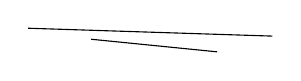
\begin{tikzpicture}[x=1cm,y=1cm]
\draw (0,0)--(3.1,-.10);\draw (.8,-.14)--(2.4,-.30);
\end{tikzpicture}}

Soit $S$ anneau avec idéal $S^+$ à p.d., muni d'un
\deleted{\unsure{suite décroissante}} $t\in S^+$.
Quitte à remplacer $S$ par son séparé complété pour la top. engendrée par les idéaux
\[
S^{[i]}=\text{idéal engendré par les }t^{(j)}\quad(j\geq i)
\]
on se suppose $S$ séparé et complet pour la top définie par une suite décroissante
d'idéaux $S^{[i]}$, chacun dans l'adhérence de l'idéal engendré par $t^{(j)}$ $(j\geq i)$.
\margin{232}

\scanpage{234}
\margin{- 189 - \qquad IX}
Donc les structures d'extension (14.1.2) et (14.1.1) peuvent
s'interpréter respectivement (VIII 3.7) comme équivalant à la donnée
d'homomorphisme
\[
(14.1.4)\qquad\underline M_K\xrightarrow{p_K}B_K,\quad
\underline M'_K\xrightarrow{p'_K}B'_K.
\]
Soient $W_K^{\natural}$ la biextension de $(B_K,B'_K)$ par $\mathbb G_{mK}$ qui définit la
dualité canonique entre ces schémas abéliens (8.2), et $E_K$ la biextension
de $(\underline M_K,\underline M'_K)$ par $\mathbb G_{mK}$ image inverse de $W_K^{\natural}$ par les homomorphismes (14.1.4).
Notons qu'on vérifie immédiatement que les trivialisations de $E_K$ correspondent
biunivoquement, de façon canonique, aux homomorphismes
\[
(14.1.5)\qquad i:\underline M_K\longrightarrow G_K
\]
qui relèvent $p_K:\underline M_K\longrightarrow B_K$, ou, symétriquement, aux homomorphismes
\[
(14.1.6)\qquad i':\underline M'_K\longrightarrow G'_K
\]
qui relèvent $P'_K:\underline M'_K\longrightarrow B'_K$.

Ceci posé, désignant par un exposant $^{\mathrm{an}}$ les groupes rigide-analytiques
sur $K$ associés aux groupes algébriques envisagés [13],
on définit dans [24] une suite exacte canonique
\[
(14.1.7)\qquad0\longrightarrow\underline M_K^{\mathrm{an}}
\xrightarrow{i^{\mathrm{an}}}G_K^{\mathrm{an}}\xrightarrow{e}A_K^{\mathrm{an}}\longrightarrow0,
\]
dans laquelle l'homomorphisme $i^{\mathrm{an}}$, qui peut aussi s'interpréter comme
un homomorphisme $i:\underline M_K\longrightarrow G_K$ pour des schémas en groupes ordinaires,
\uline{relève l'homomorphisme} $p$ (14.1.4), i.e. est de la forme envisagée dans
(14.1.5). Cette suite exacte est l'analogue rigide-analytique de la
suite exacte (13.3.4). Elle dépend de façon fonctorielle de $A_K$, et
\margin{507}
\margin{507}
\margin{233}
